% Chapter Template

\chapter{Datos: Sólo datos.} % Main chapter title

\label{Cap_Data} % Change X to a consecutive number; for referencing this chapter elsewhere, use \ref{ChapterX}

%----------------------------------------------------------------------------------------
%	SECTION 1
%----------------------------------------------------------------------------------------
\section{Explorando la ejecución de los participantes}



\subsection{Control 1: ¿Los participantes estaban poniendo atención a la tarea?}

Lorem ipsum dolor sit amet, consectetur adipiscing elit. Aliquam ultricies lacinia euismod. Nam tempus risus in dolor rhoncus in interdum enim tincidunt. Donec vel nunc neque. In condimentum ullamcorper quam non consequat. Fusce sagittis tempor feugiat. Fusce magna erat, molestie eu convallis ut, tempus sed arcu. Quisque molestie, ante a tincidunt ullamcorper, sapien enim dignissim lacus, in semper nibh erat lobortis purus. Integer dapibus ligula ac risus convallis pellentesque.


%%%%%%%%%%%%%%%%%%%%%%%%%%%%%%%%%%%%%%%%%%%%%%%%%%%%%%%%%%%%%%
%%%%%%%%%  Respuesta (Y/N) en los ensayos
% Experimento 2
%%%%%%%%%%%%%%%%%%%%%%%%%%%%%%%%%%%%%%%%%%%%%%%%%%%%%%%%%%%%%%%
\begin{figure}[th]
\centering
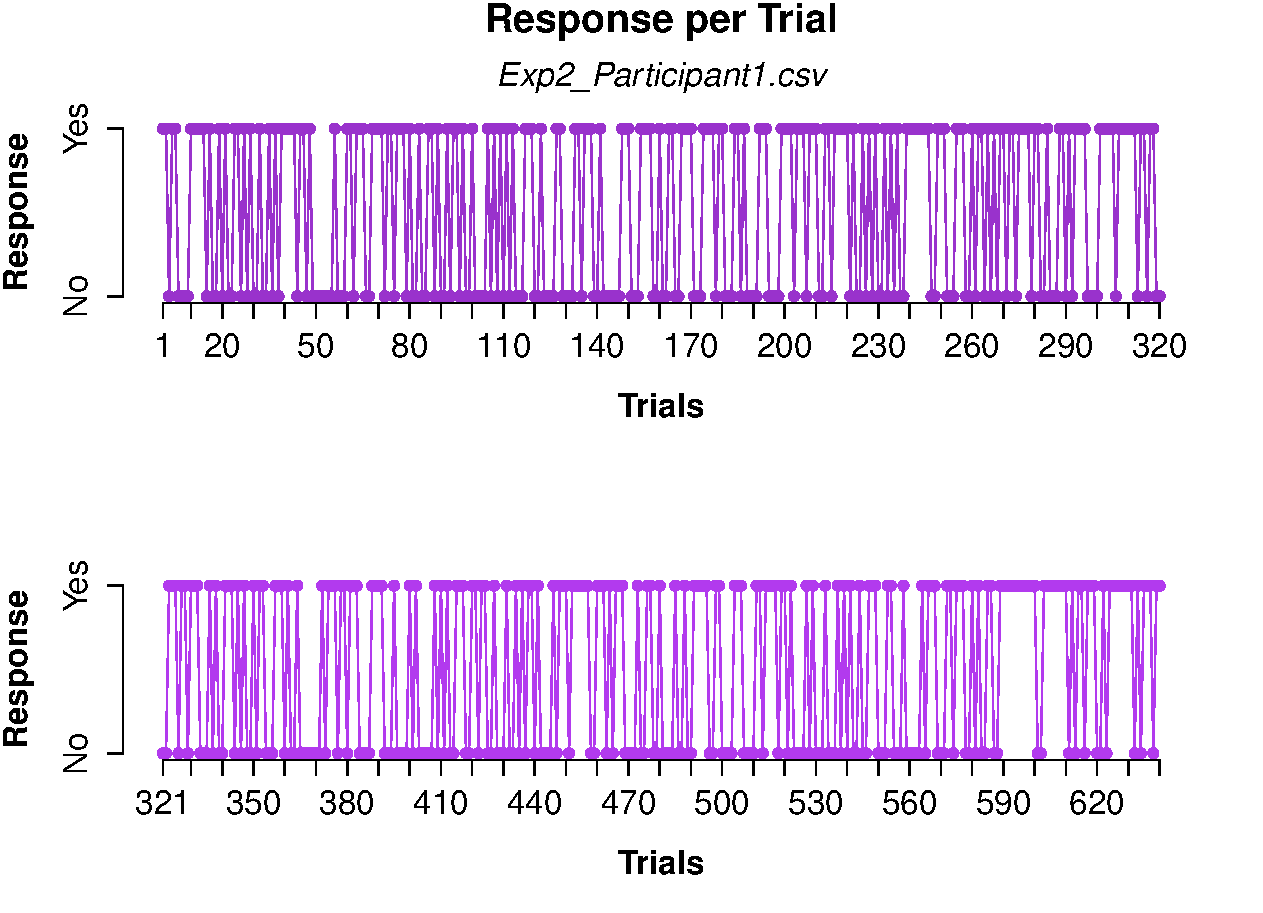
\includegraphics[width=0.30\textwidth]{Figures/Response_Exp2_P1} 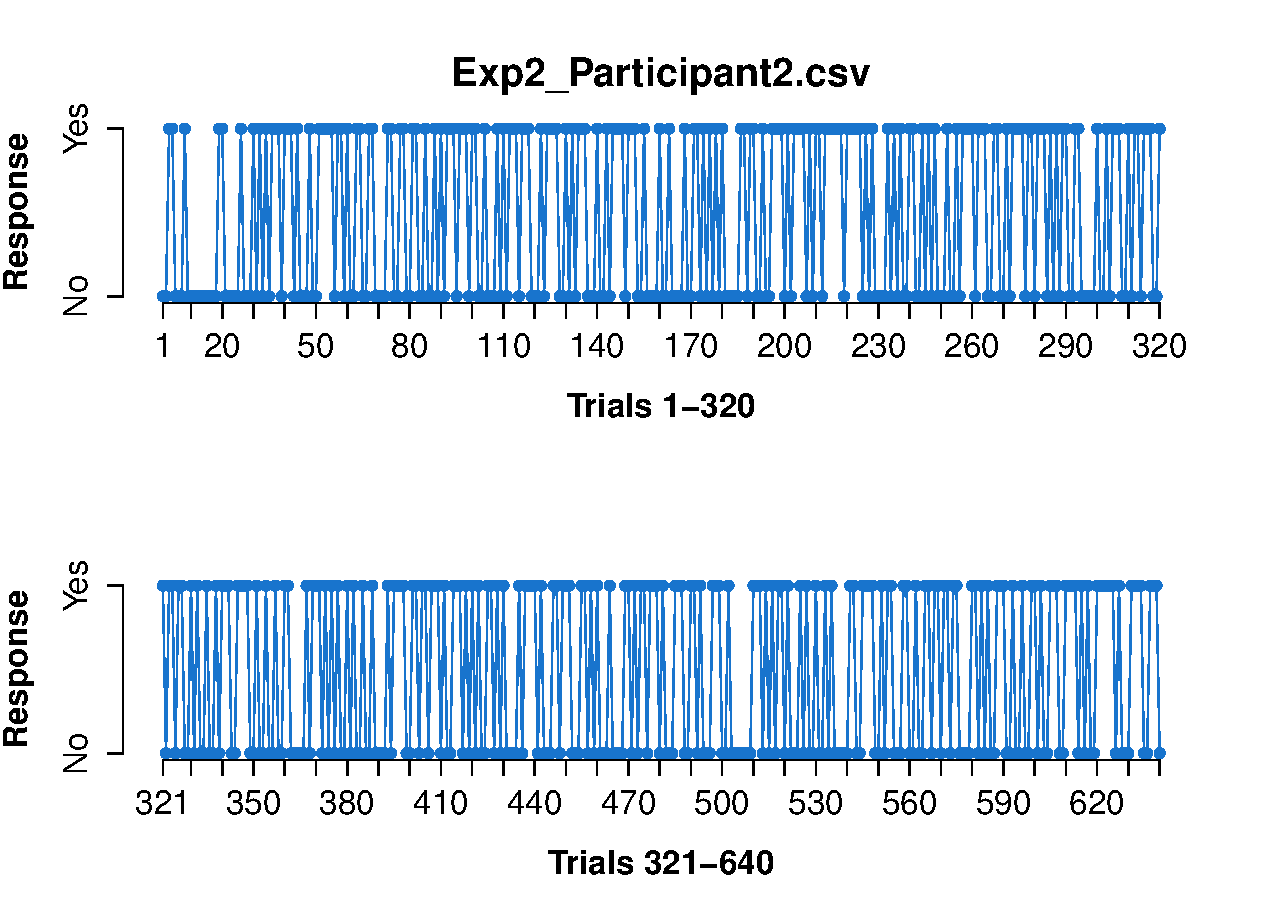
\includegraphics[width=0.30\textwidth]{Figures/Response_Exp2_P2} 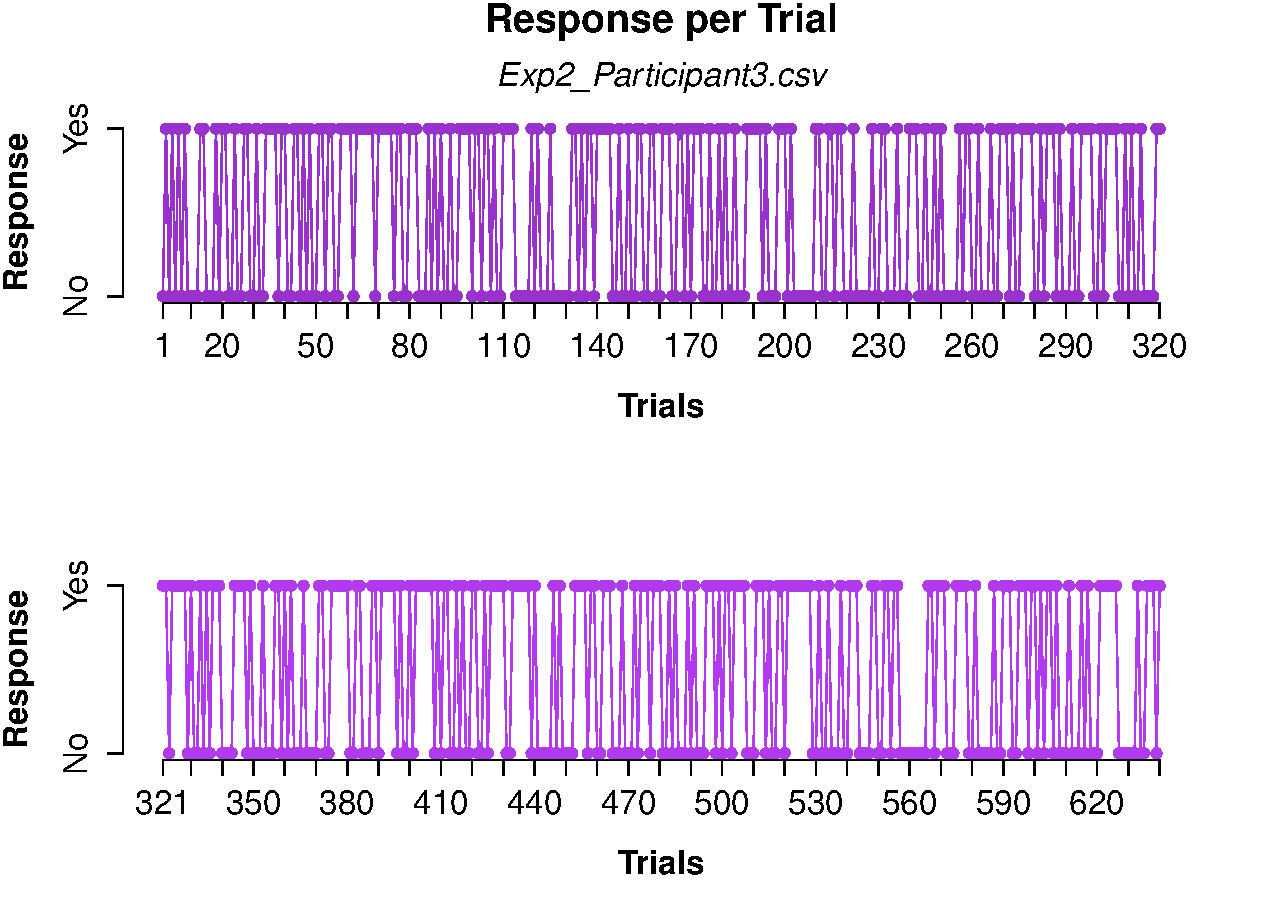
\includegraphics[width=0.30\textwidth]{Figures/Response_Exp2_P3}
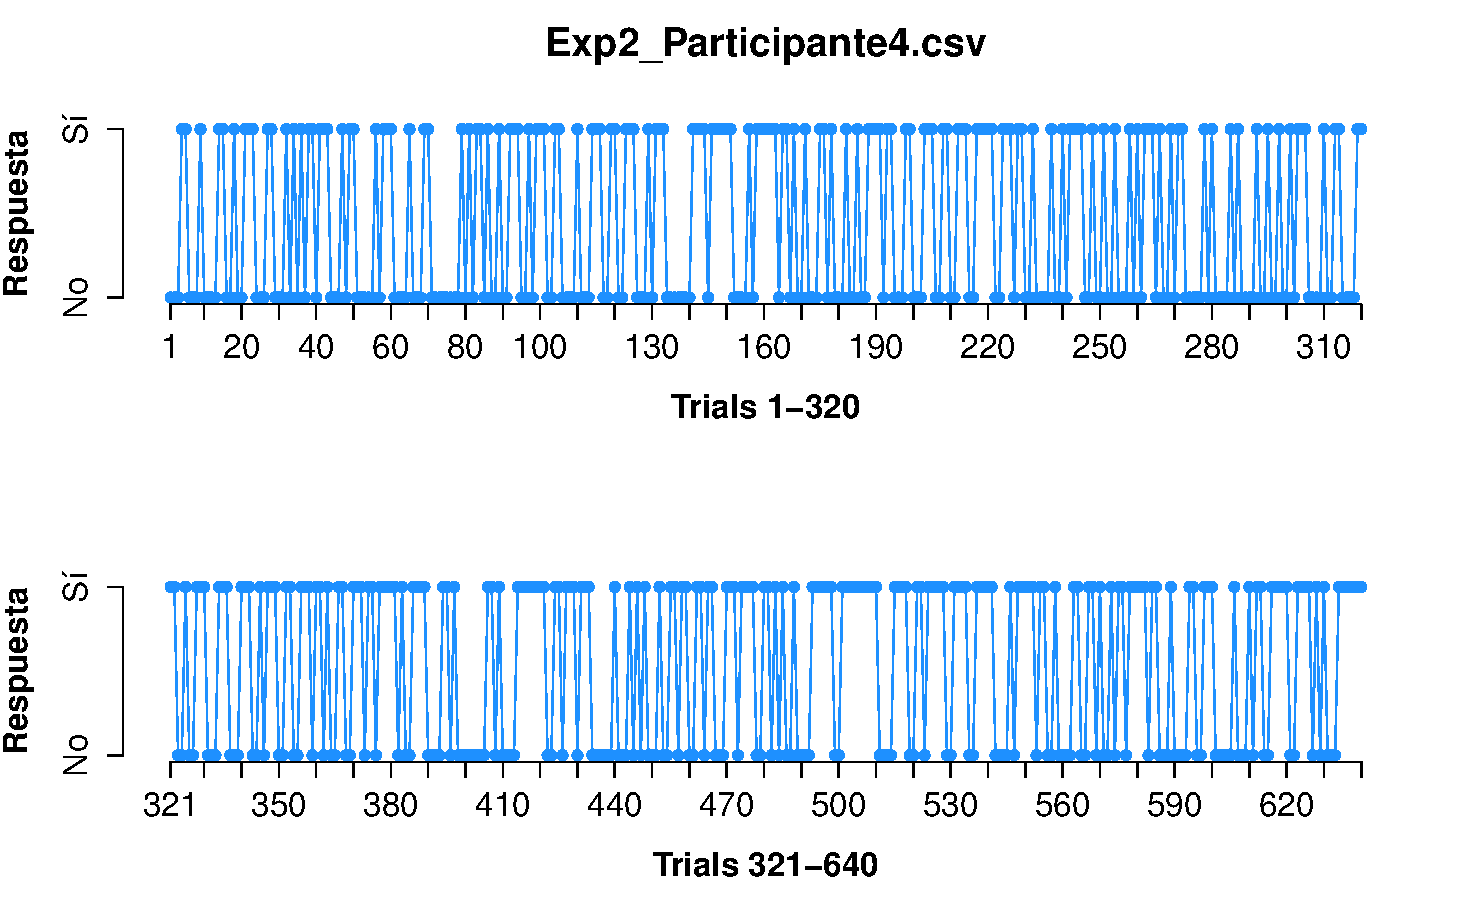
\includegraphics[width=0.30\textwidth]{Figures/Response_Exp2_P4} 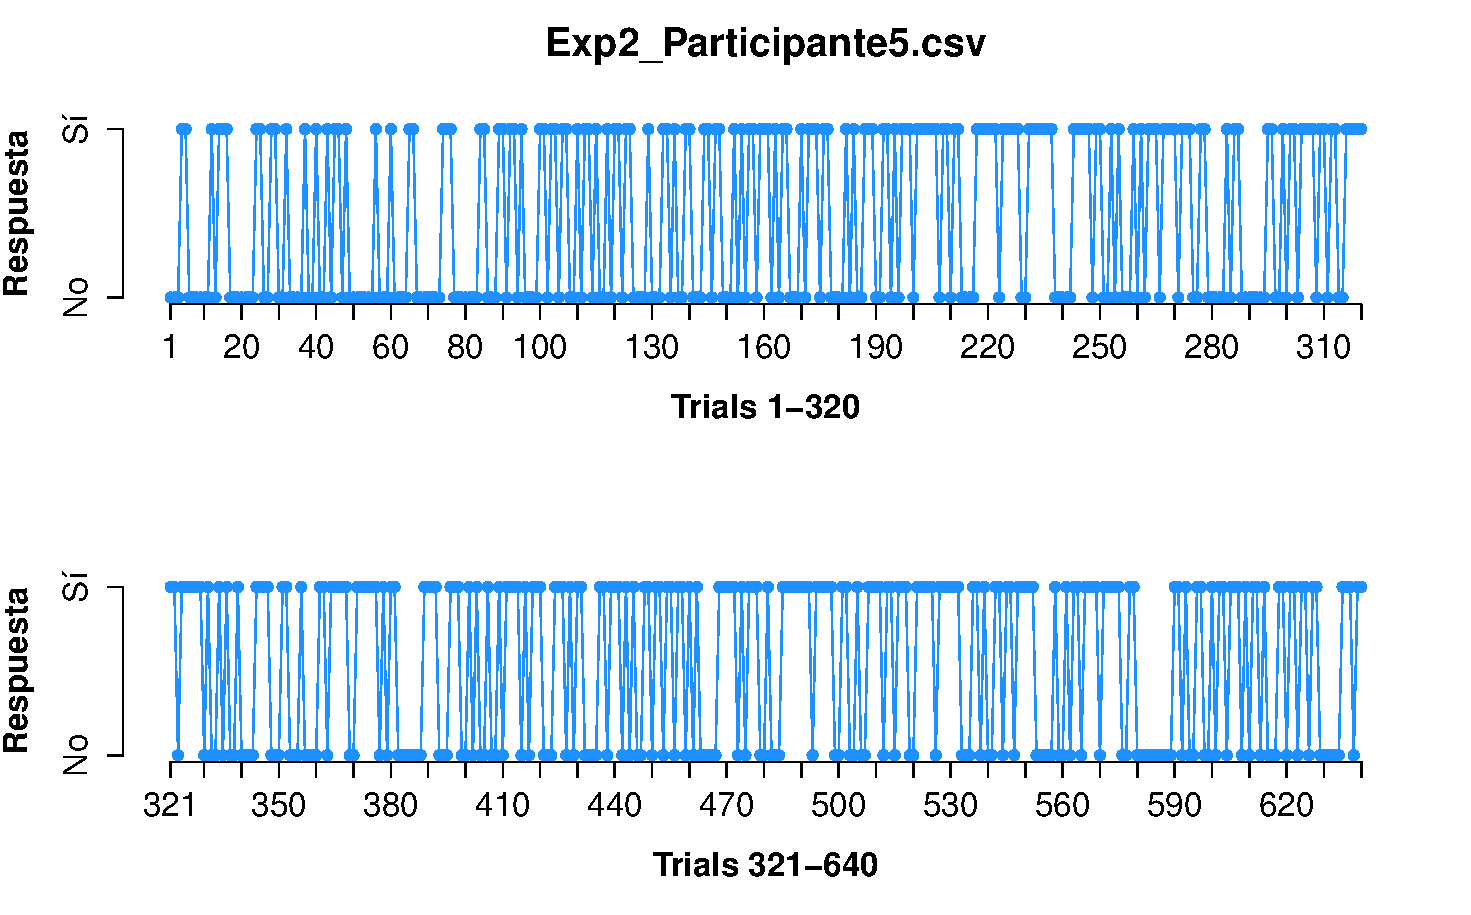
\includegraphics[width=0.30\textwidth]{Figures/Response_Exp2_P5} 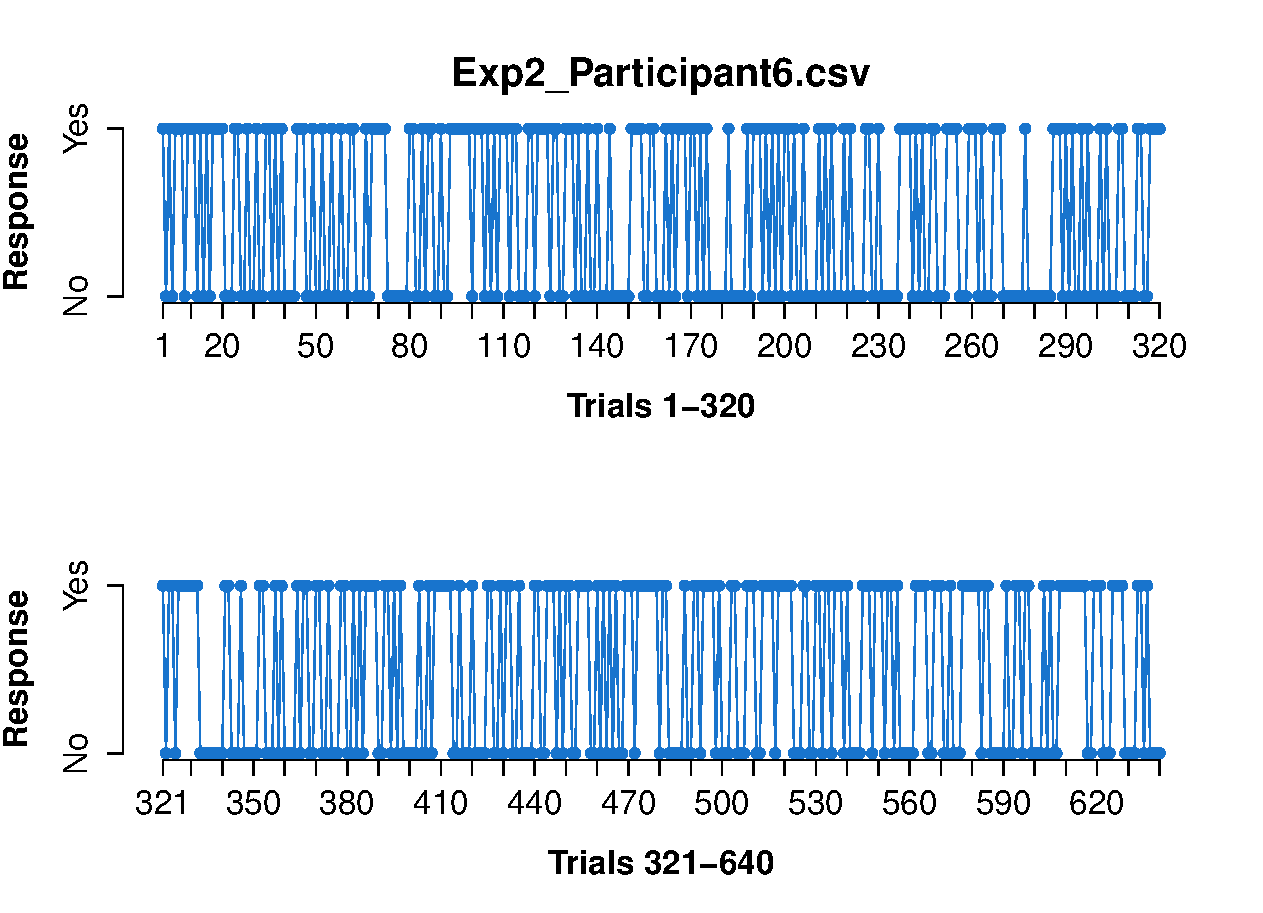
\includegraphics[width=0.30\textwidth]{Figures/Response_Exp2_P6}
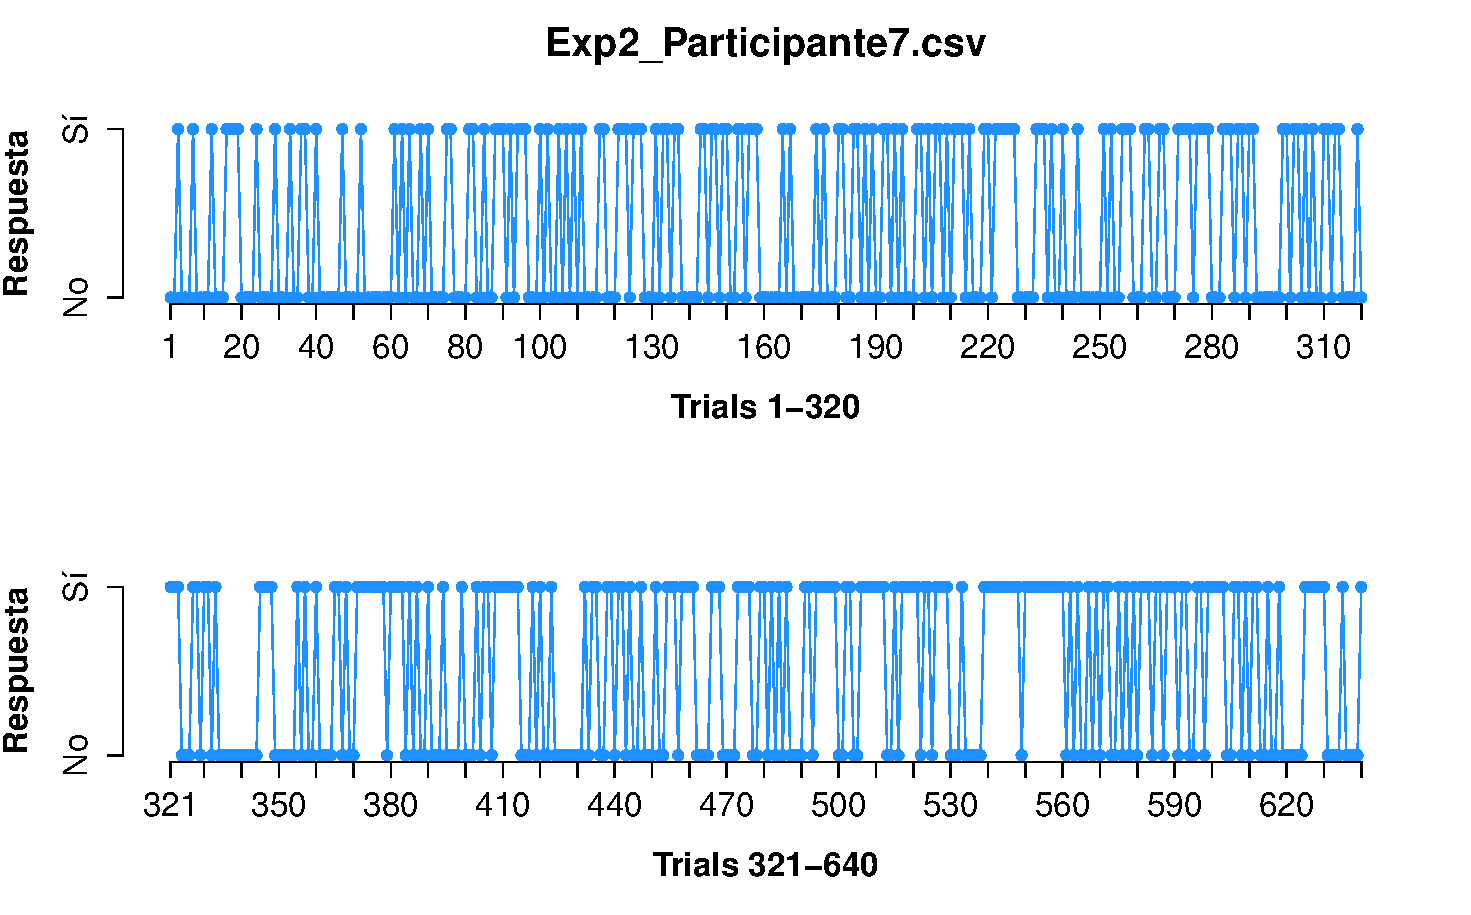
\includegraphics[width=0.30\textwidth]{Figures/Response_Exp2_P7} 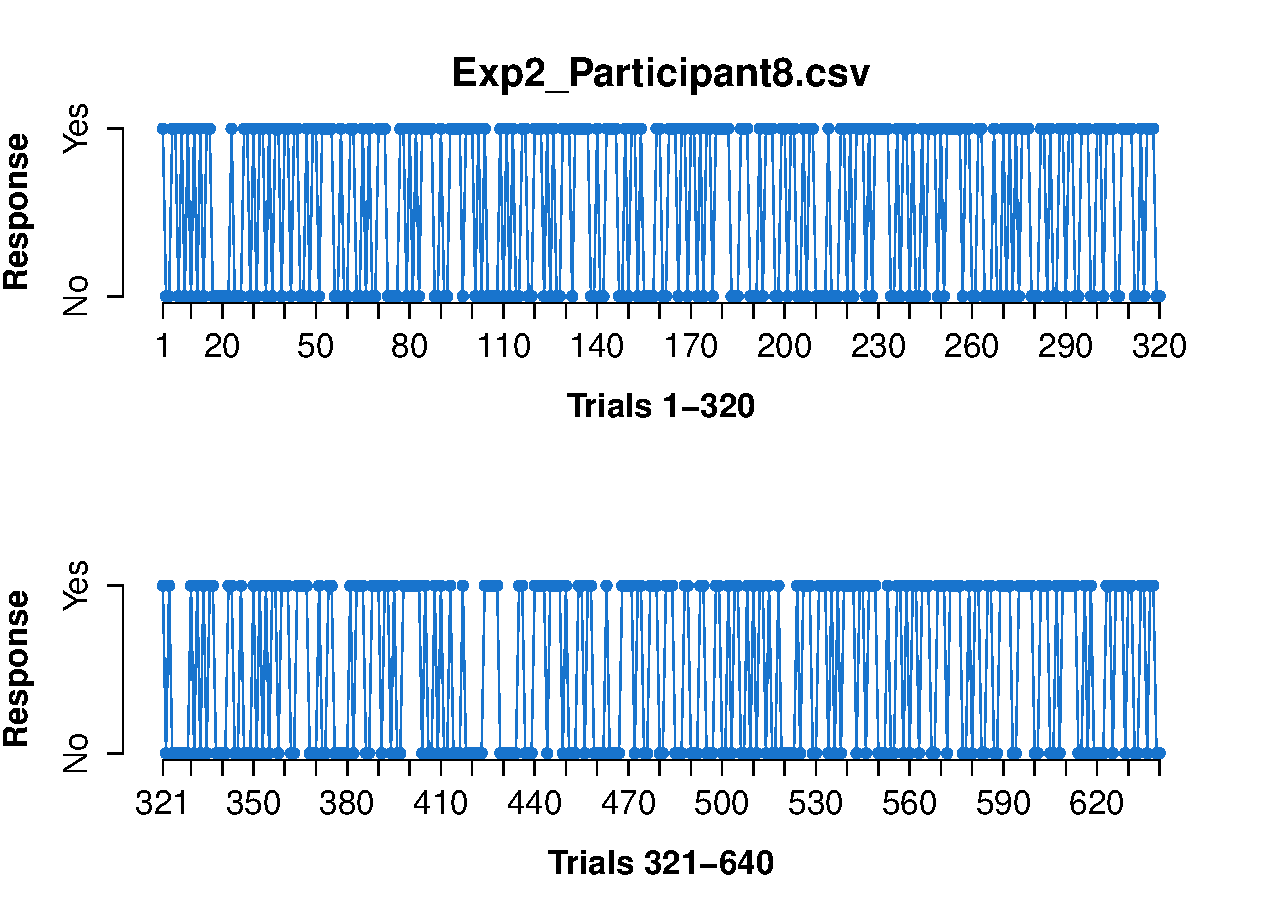
\includegraphics[width=0.30\textwidth]{Figures/Response_Exp2_P8} 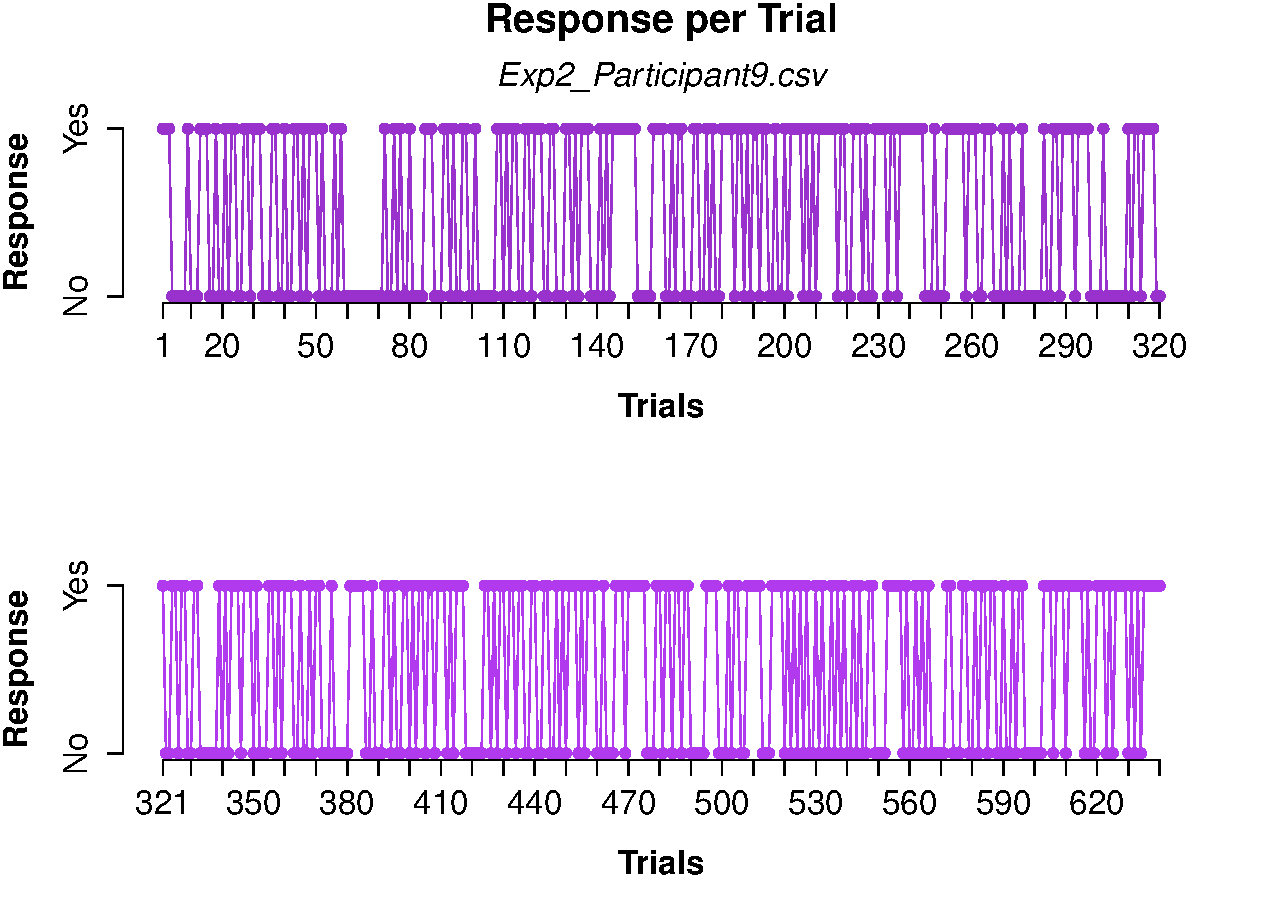
\includegraphics[width=0.30\textwidth]{Figures/Response_Exp2_P9}
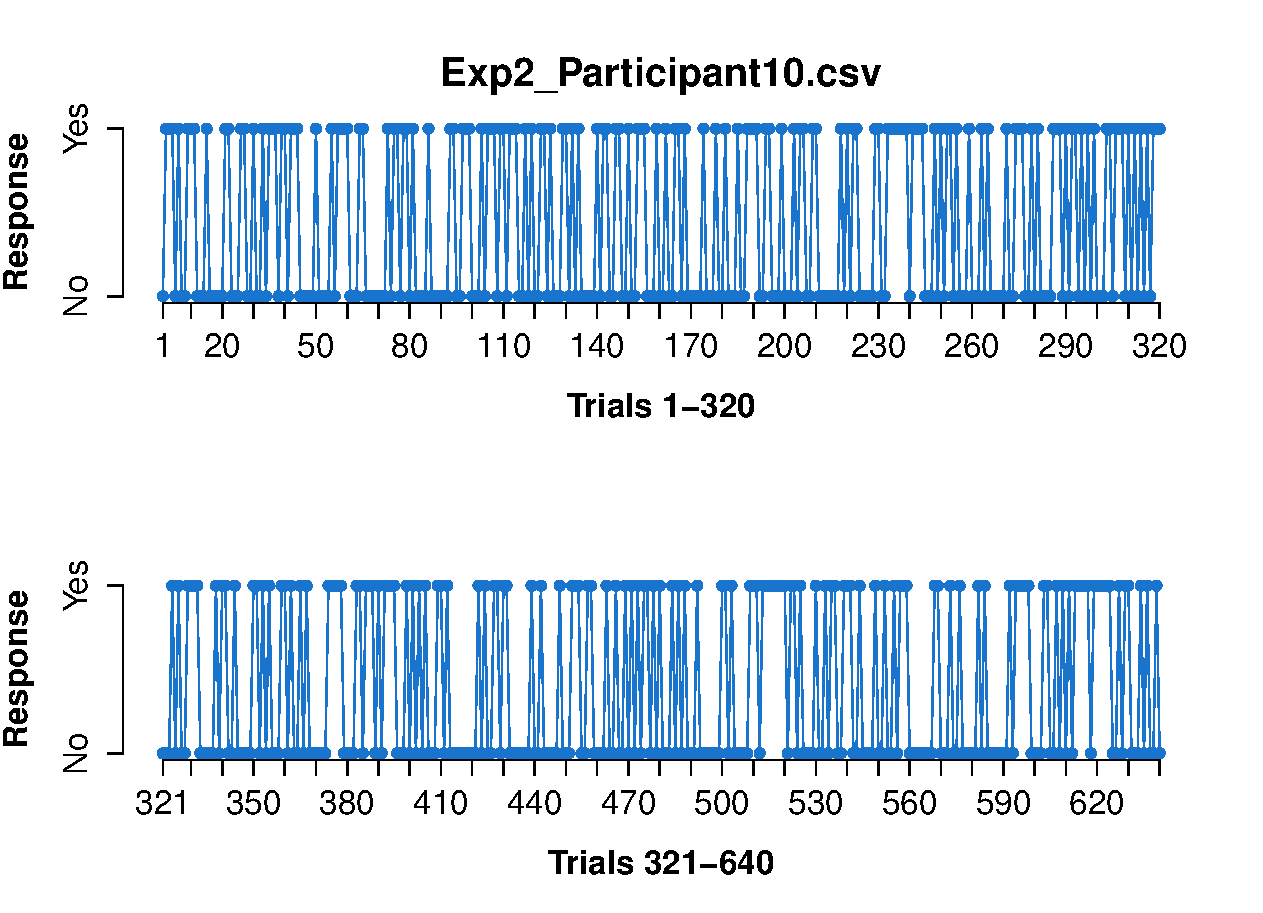
\includegraphics[width=0.30\textwidth]{Figures/Response_Exp2_P10} 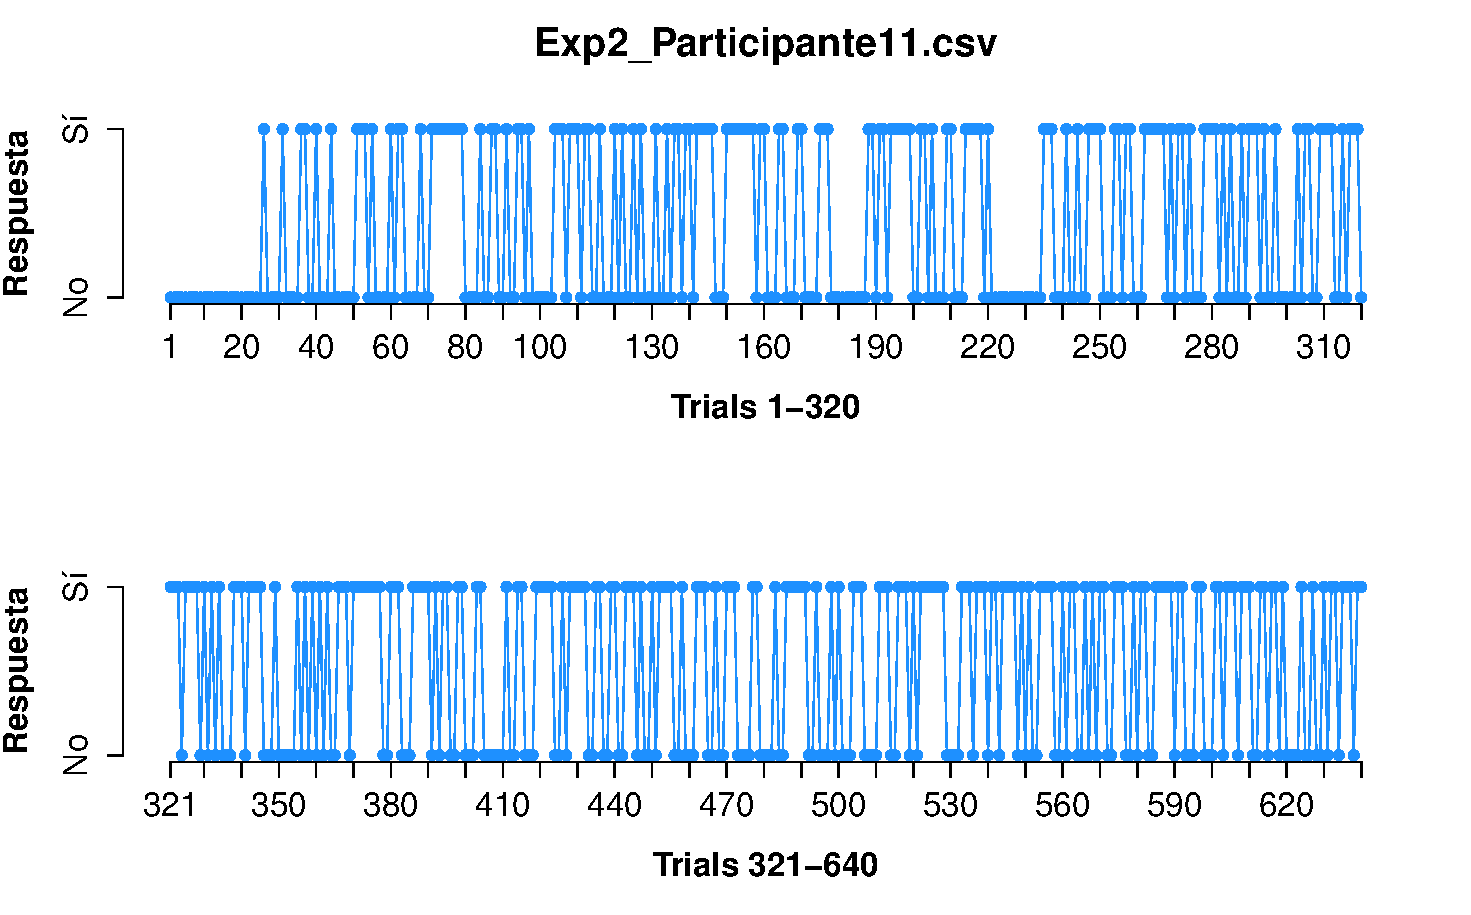
\includegraphics[width=0.30\textwidth]{Figures/Response_Exp2_P11} 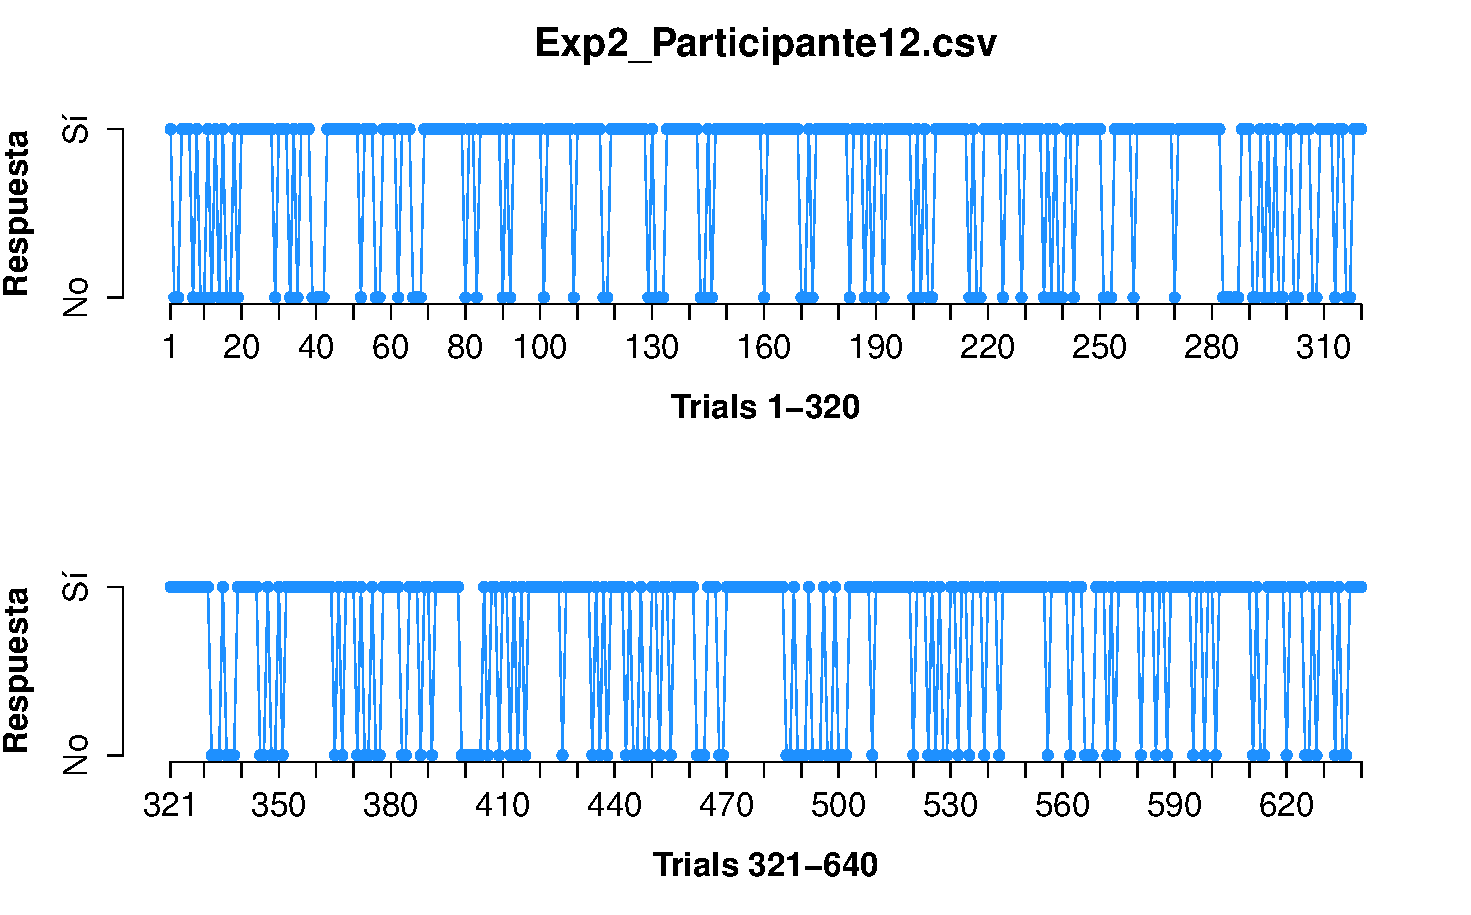
\includegraphics[width=0.30\textwidth]{Figures/Response_Exp2_P12}
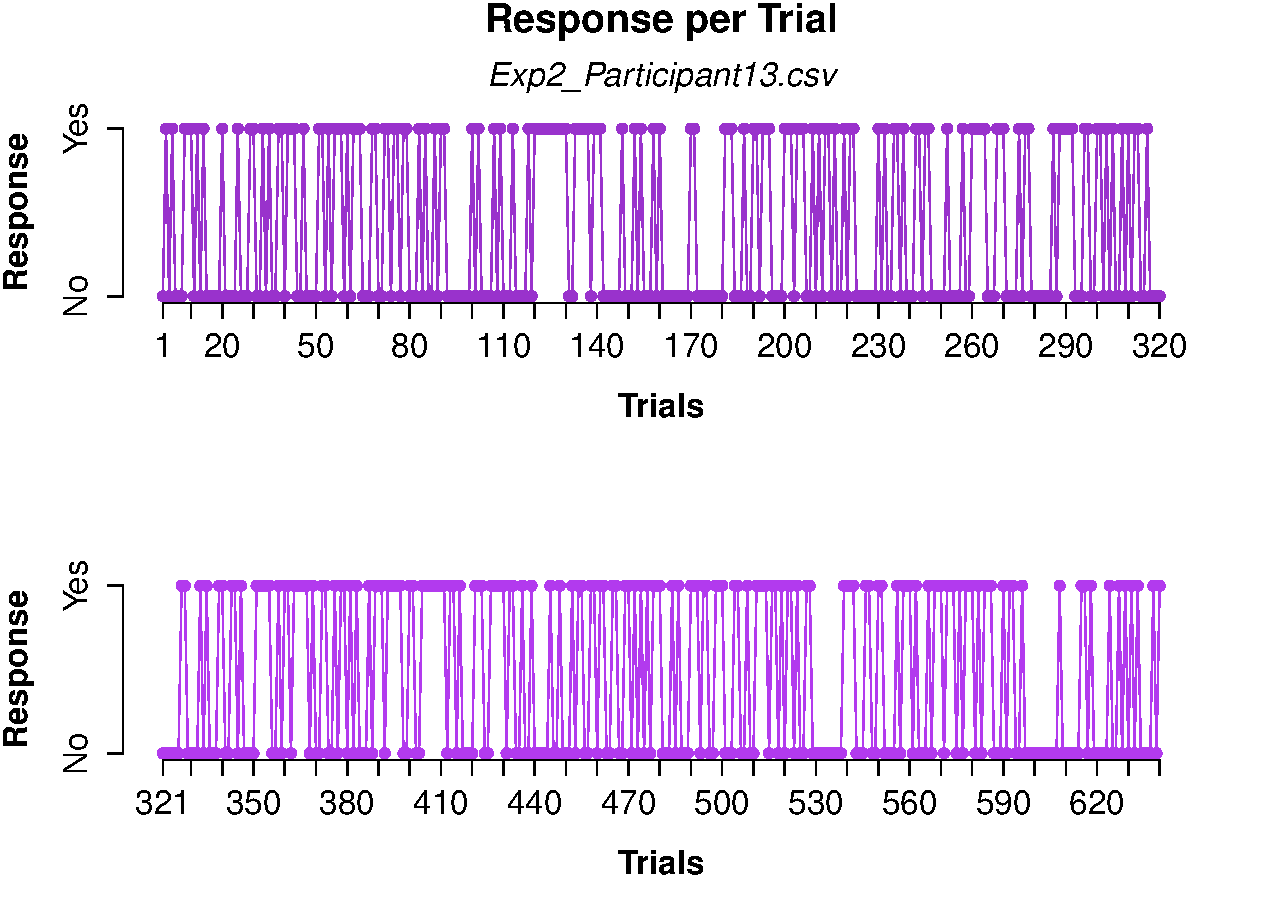
\includegraphics[width=0.30\textwidth]{Figures/Response_Exp2_P13} 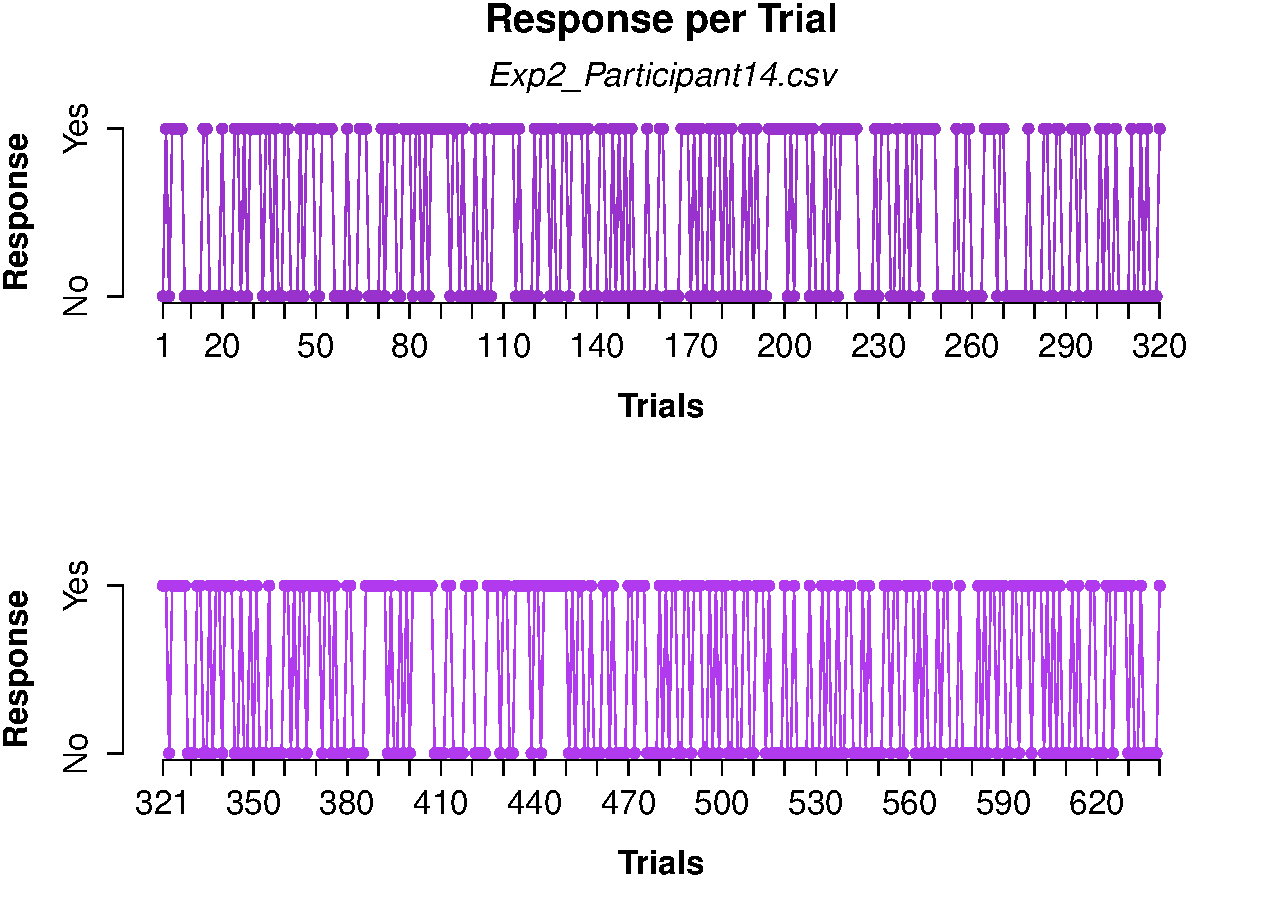
\includegraphics[width=0.30\textwidth]{Figures/Response_Exp2_P14} 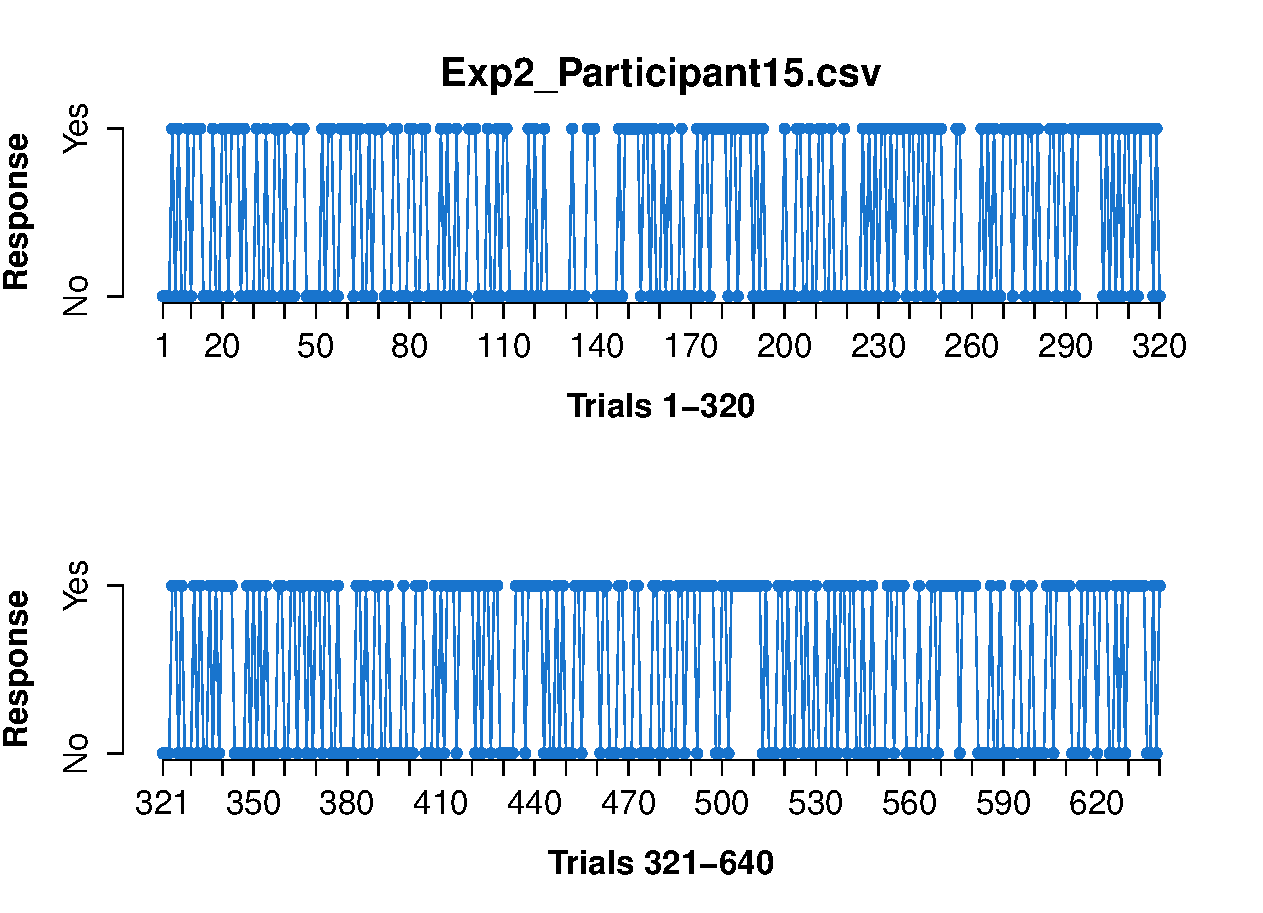
\includegraphics[width=0.30\textwidth]{Figures/Response_Exp2_P15}
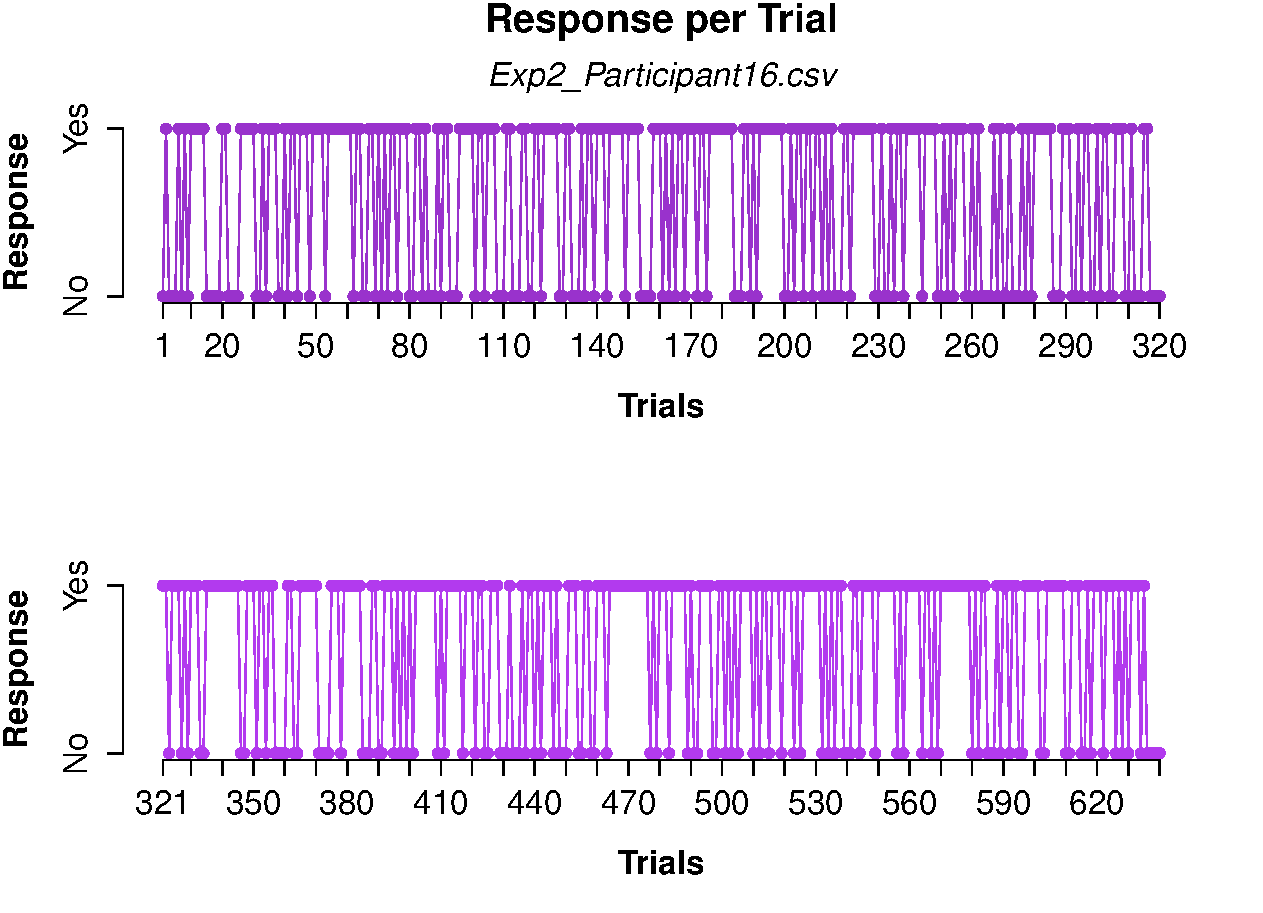
\includegraphics[width=0.30\textwidth]{Figures/Response_Exp2_P16} 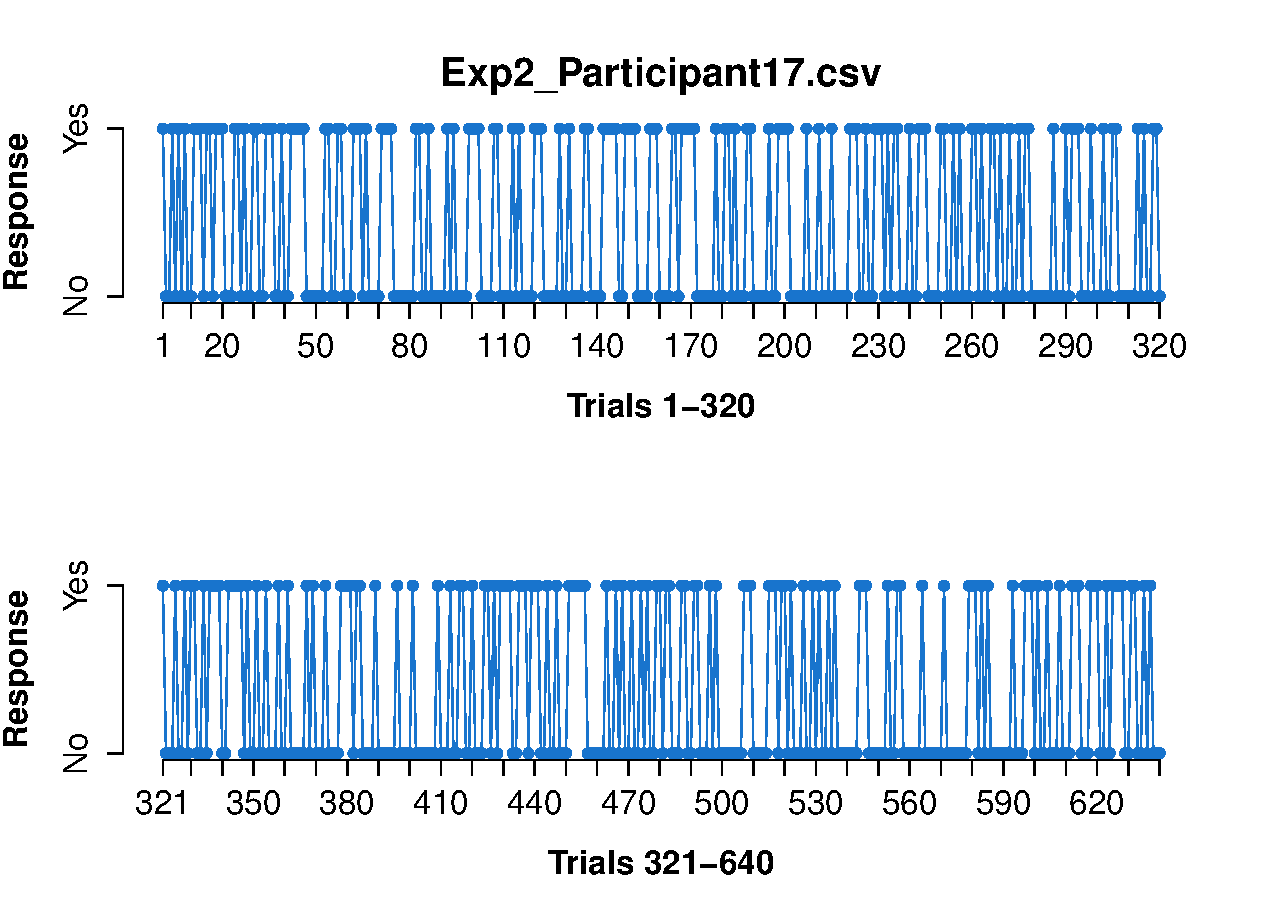
\includegraphics[width=0.30\textwidth]{Figures/Response_Exp2_P17} 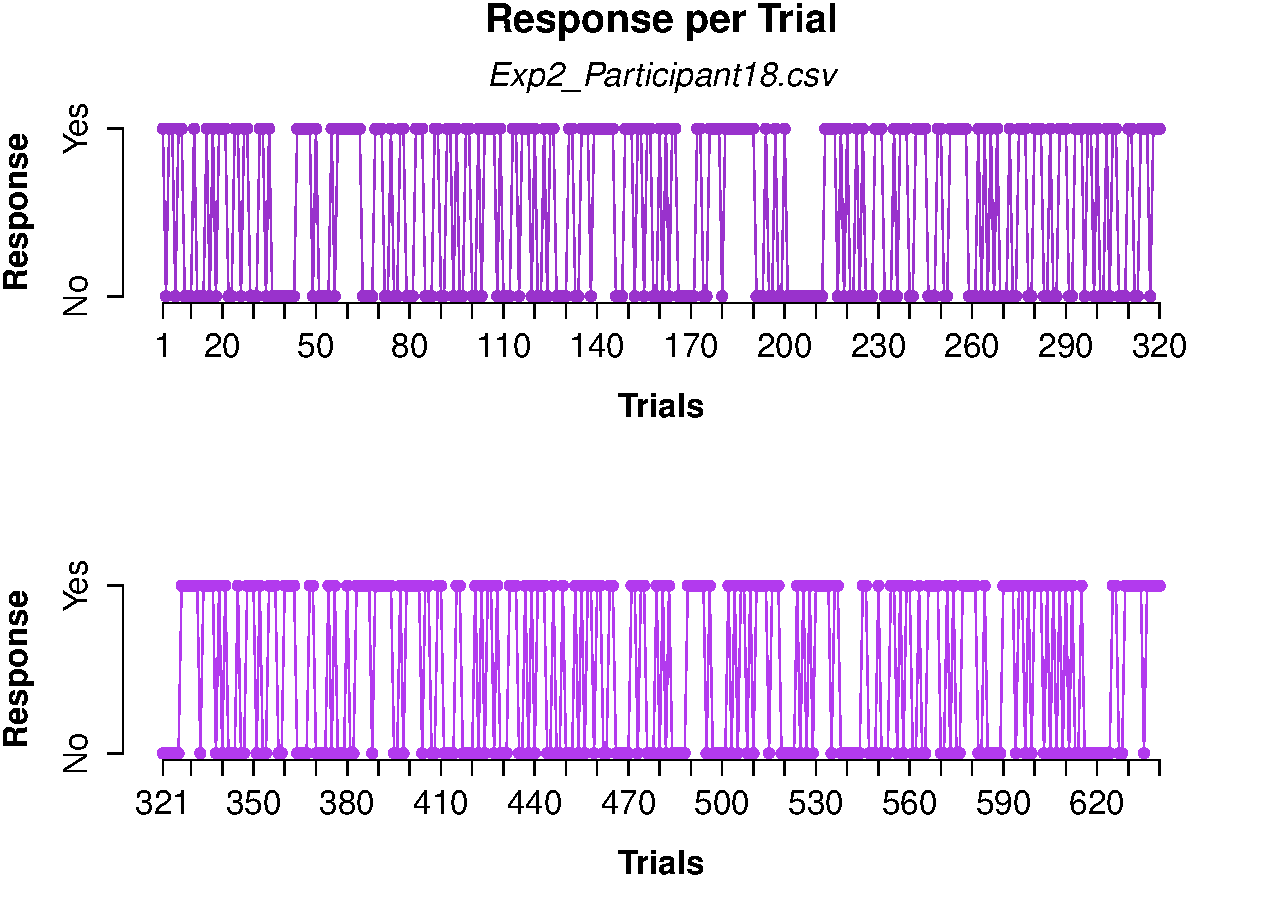
\includegraphics[width=0.30\textwidth]{Figures/Response_Exp2_P18}
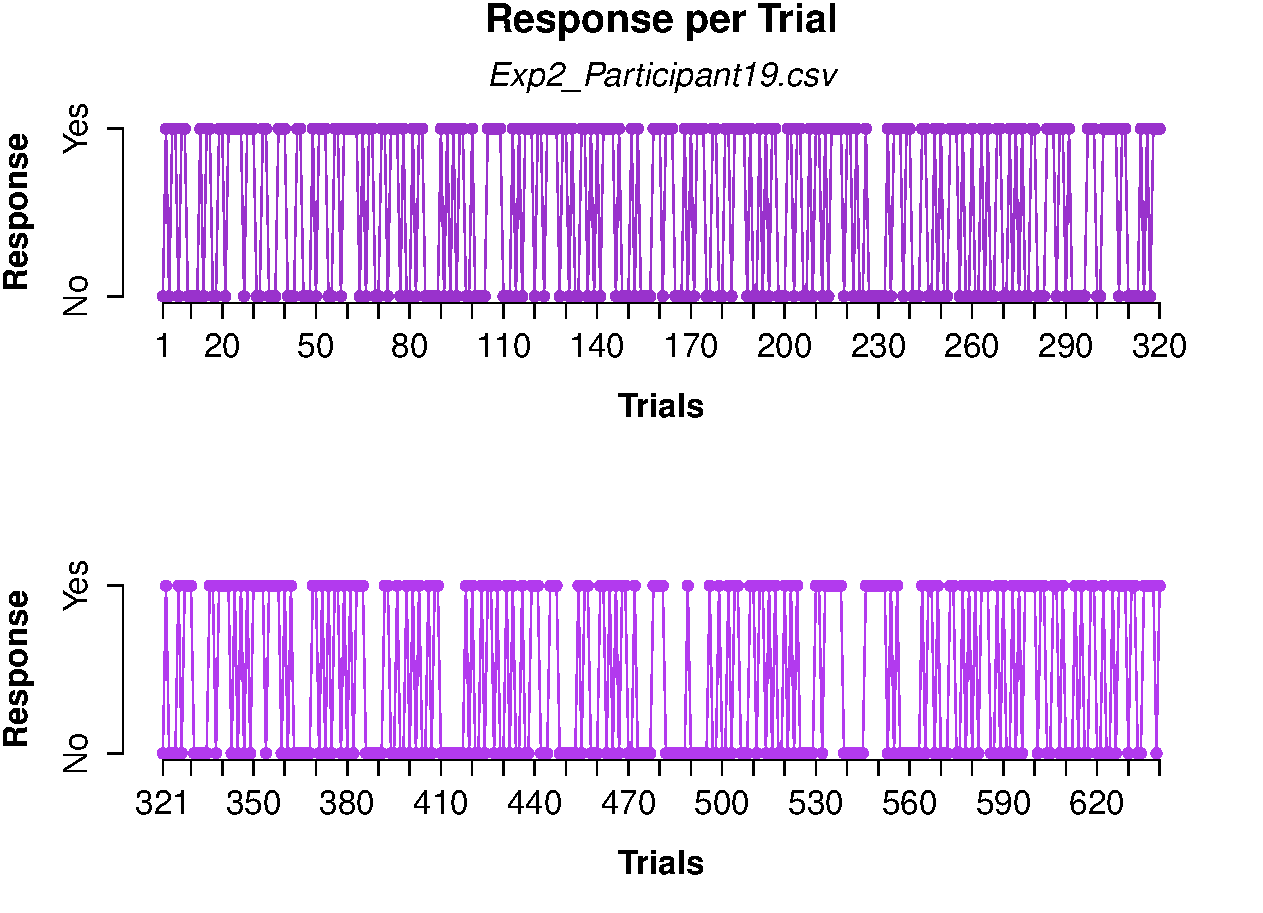
\includegraphics[width=0.30\textwidth]{Figures/Response_Exp2_P19} 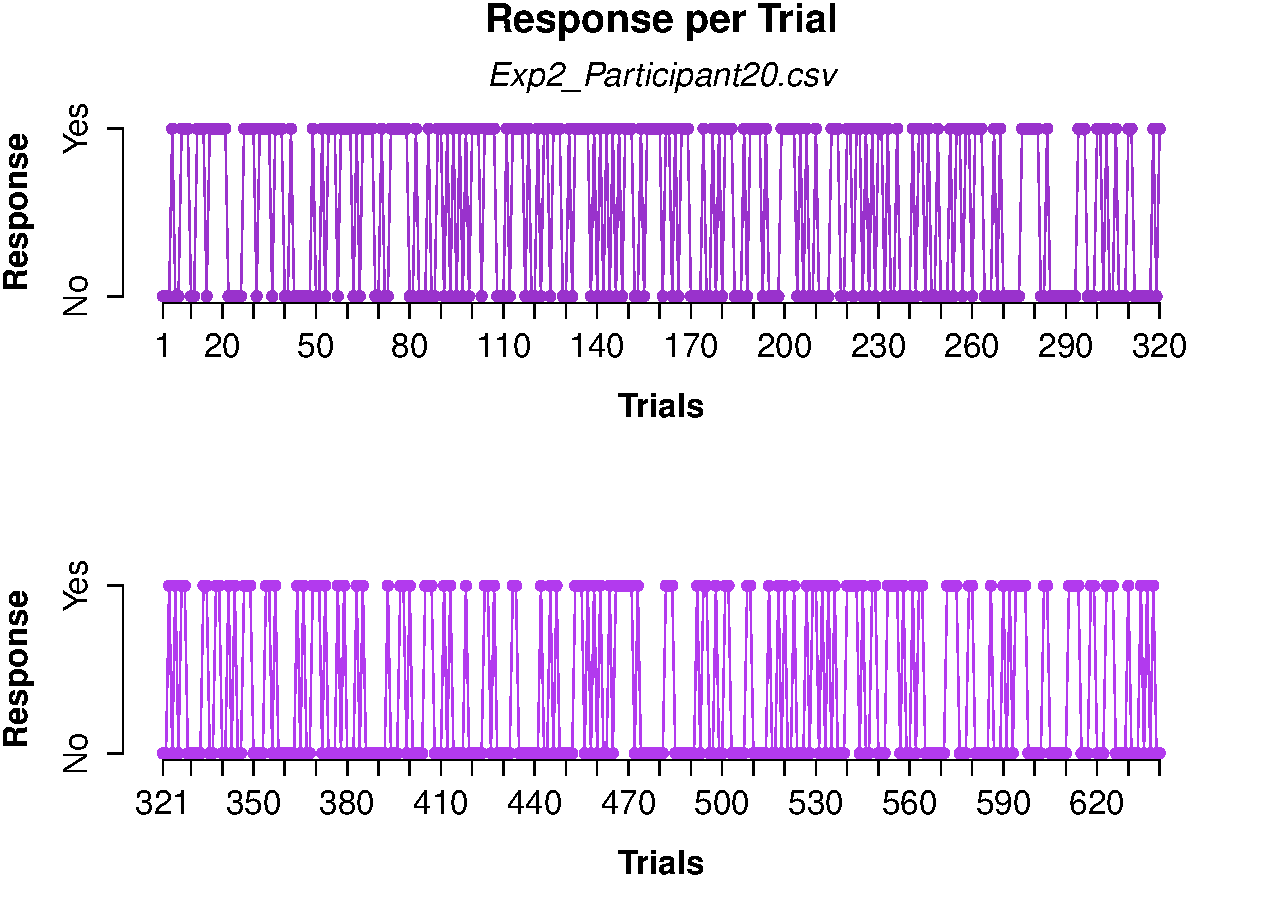
\includegraphics[width=0.30\textwidth]{Figures/Response_Exp2_P20} 
%\decoRule
\caption[Response_Exp2]{Respuesta por ensayo (Experimento 2).}
\label{fig:Response_E2}
\end{figure}



%%%%%%%%%%%%%%%%%%%%%%%%%%%%%%%%%%%%%%%%%%%%%%%%%%%%%%%%%%%%%%
%%%%%%%%%  Respuesta Rating en los ensayos
% Experimento 2
%%%%%%%%%%%%%%%%%%%%%%%%%%%%%%%%%%%%%%%%%%%%%%%%%%%%%%%%%%%%%%%
\begin{figure}[th]
\centering
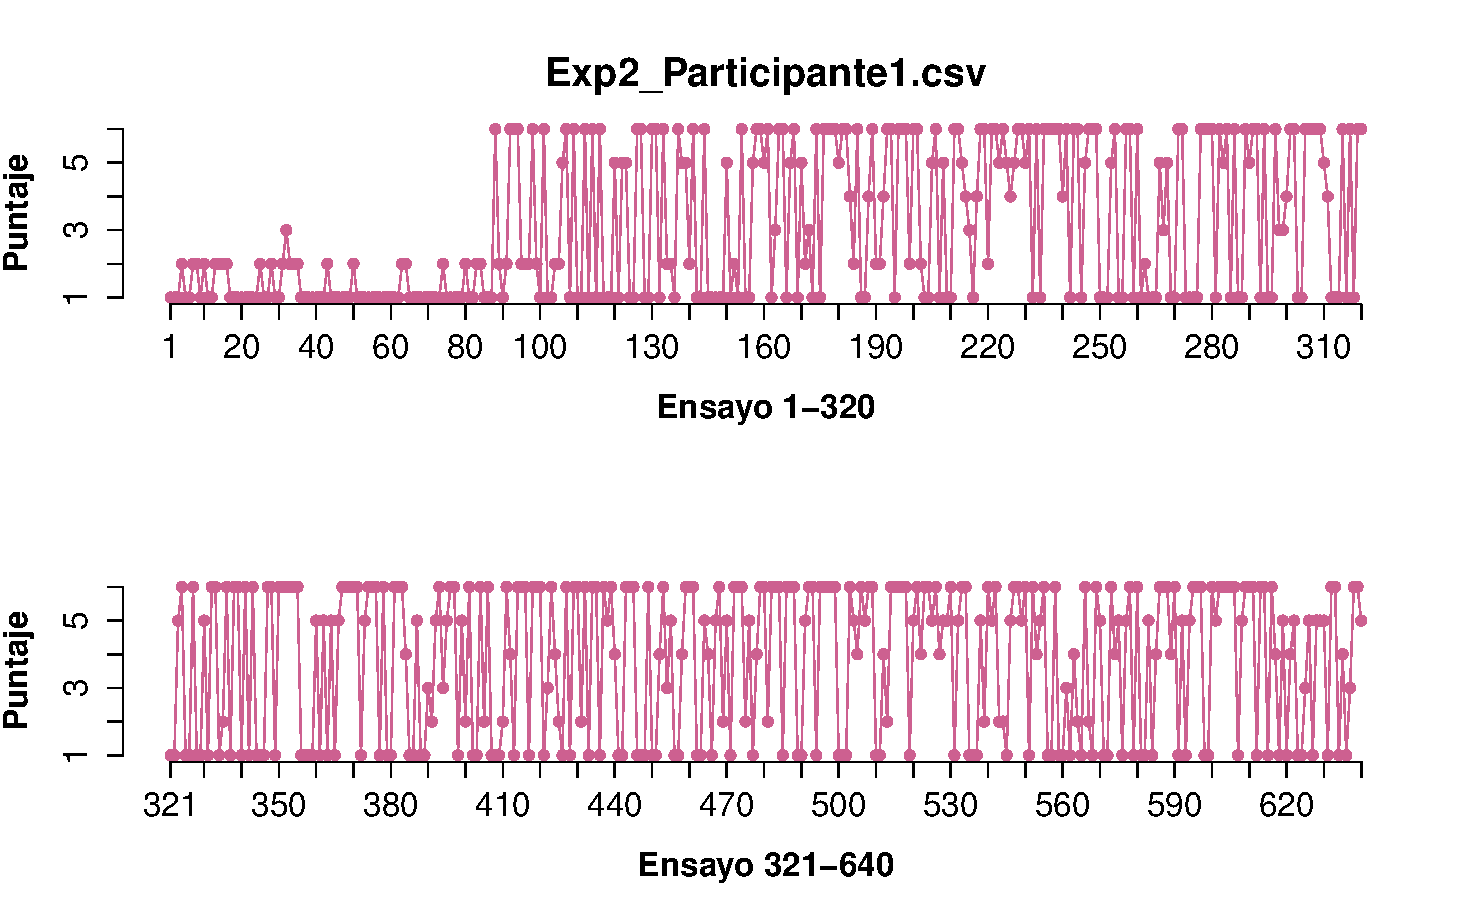
\includegraphics[width=0.30\textwidth]{Figures/Rating_Exp2_P1} 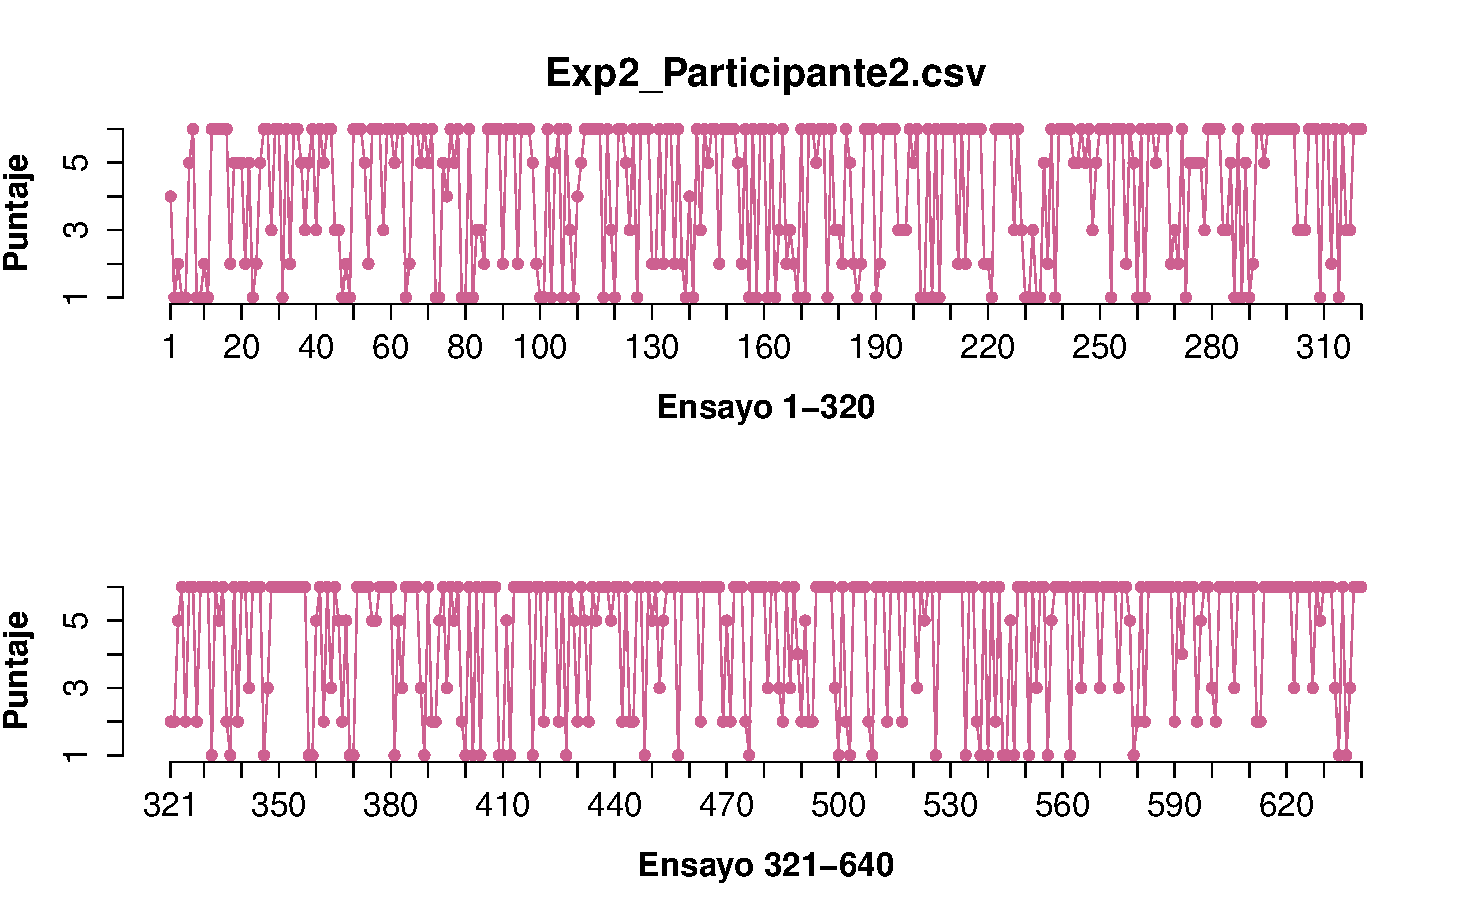
\includegraphics[width=0.30\textwidth]{Figures/Rating_Exp2_P2} 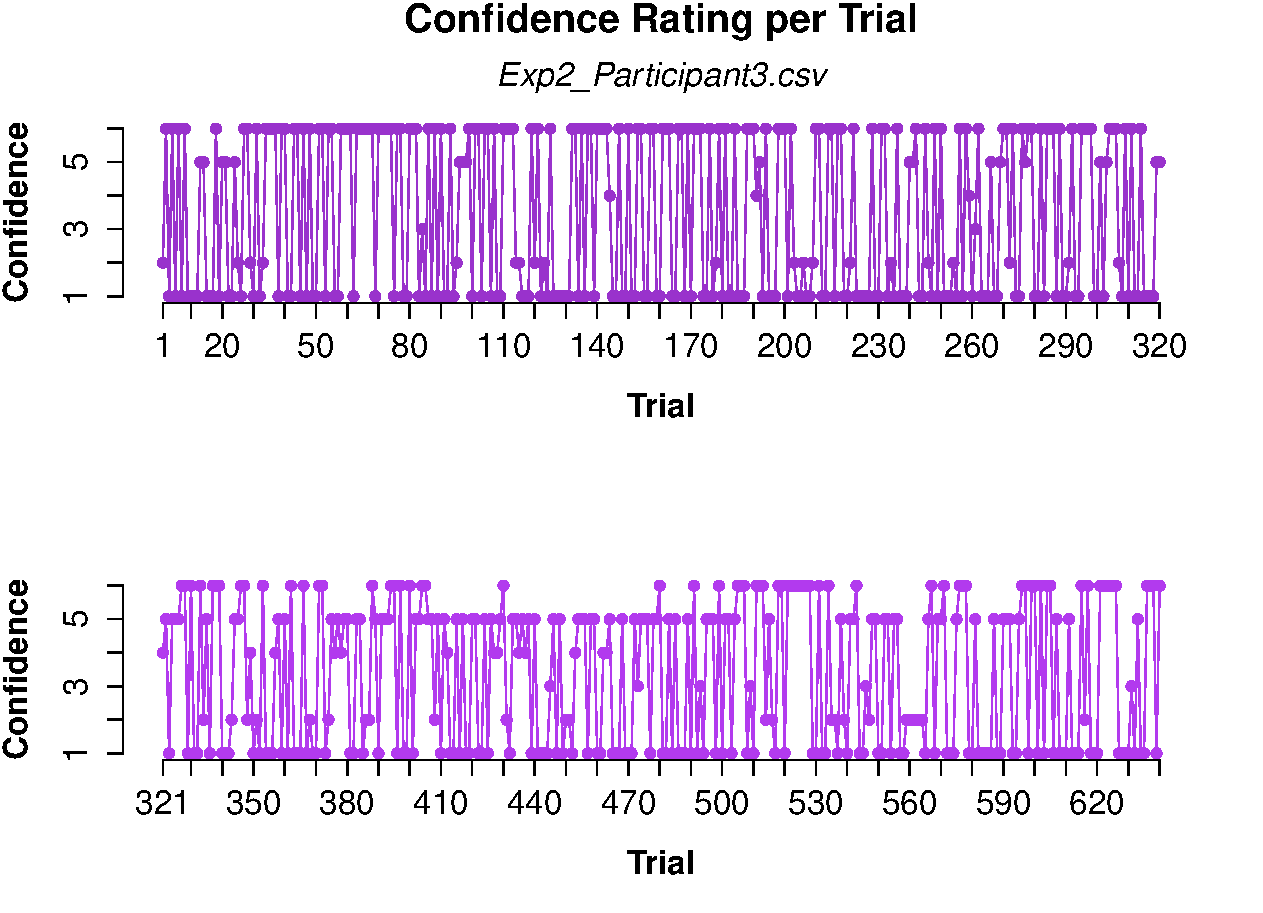
\includegraphics[width=0.30\textwidth]{Figures/Rating_Exp2_P3}
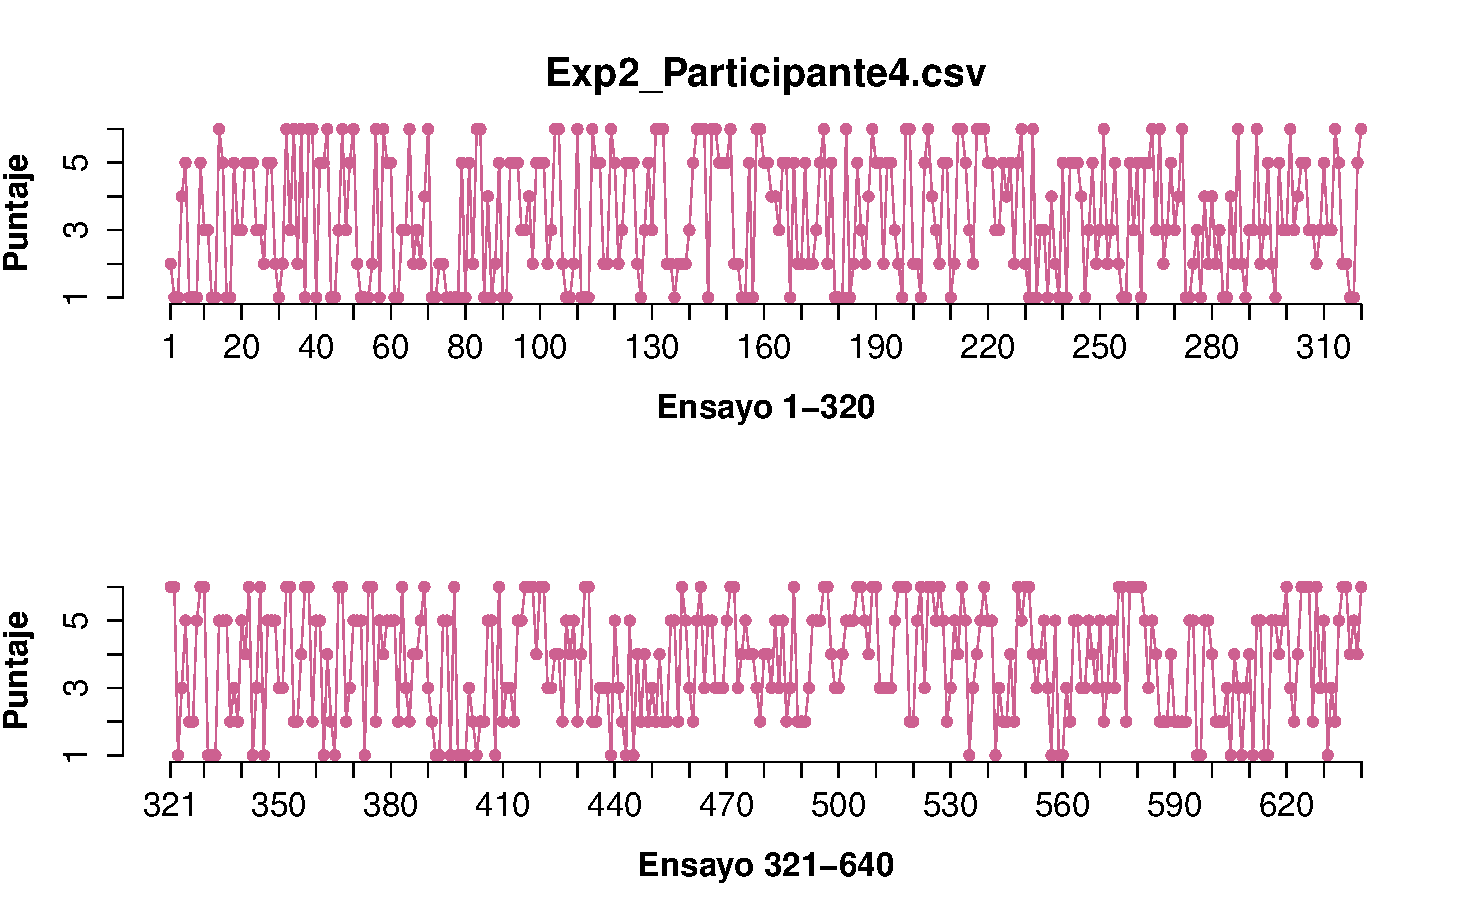
\includegraphics[width=0.30\textwidth]{Figures/Rating_Exp2_P4} 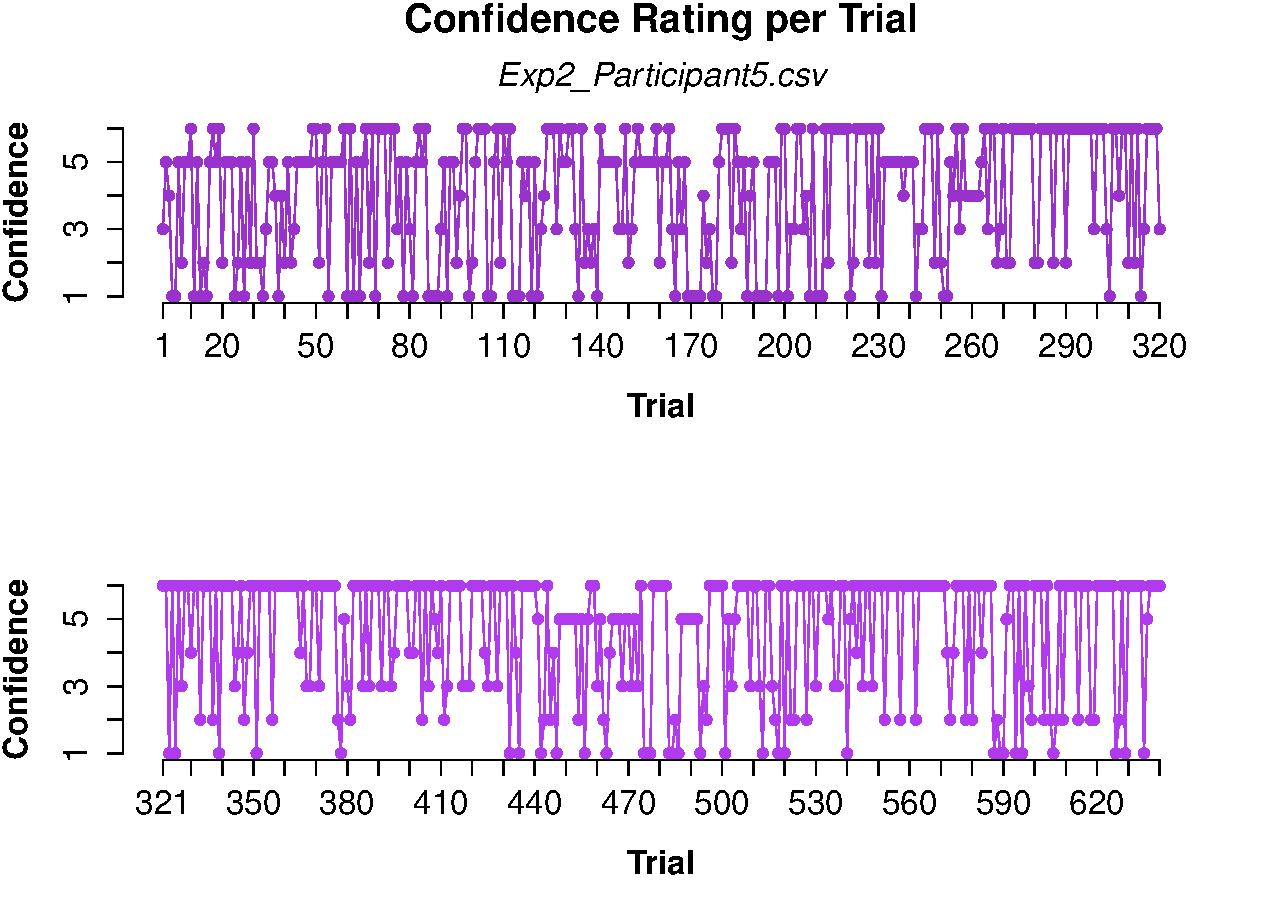
\includegraphics[width=0.30\textwidth]{Figures/Rating_Exp2_P5} 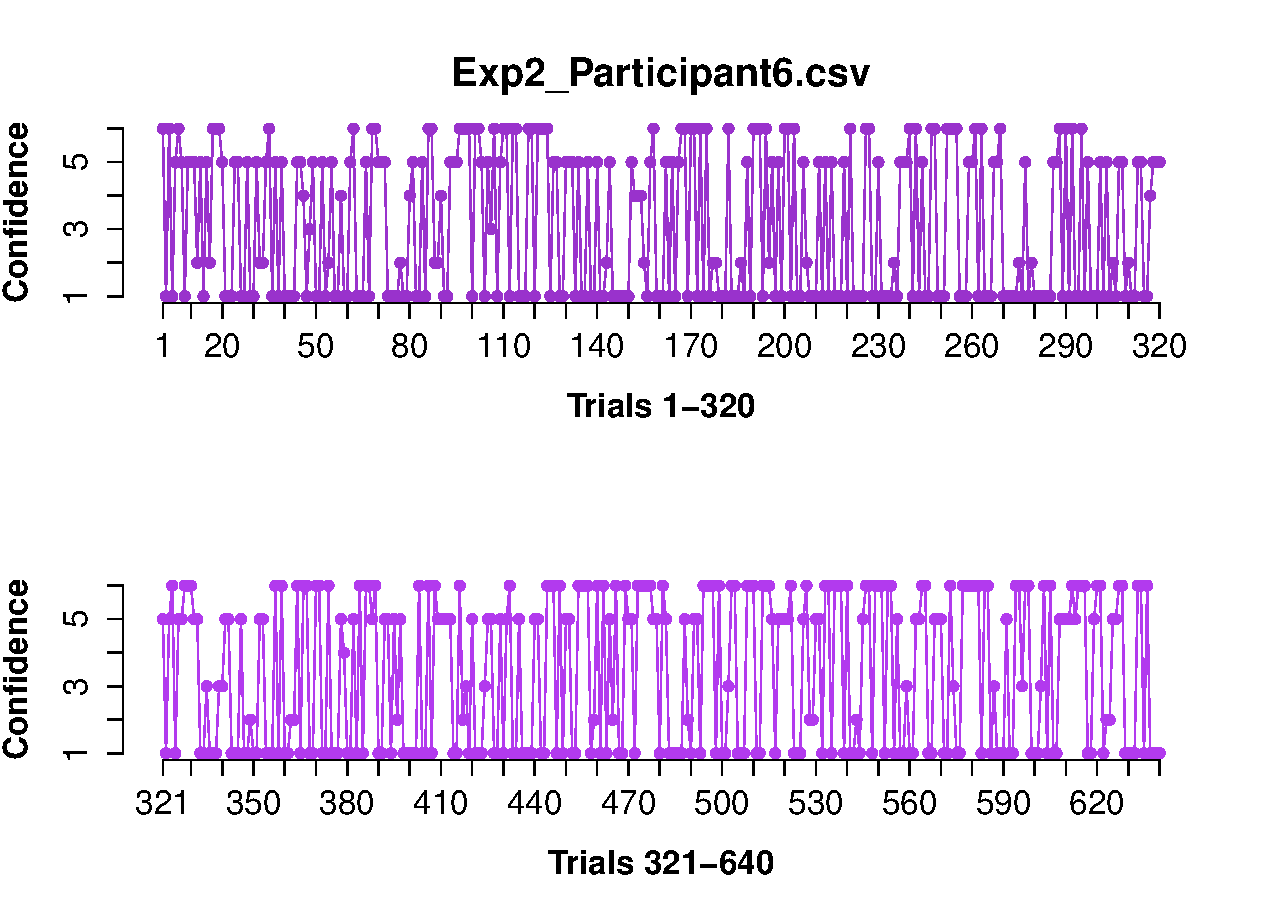
\includegraphics[width=0.30\textwidth]{Figures/Rating_Exp2_P6}
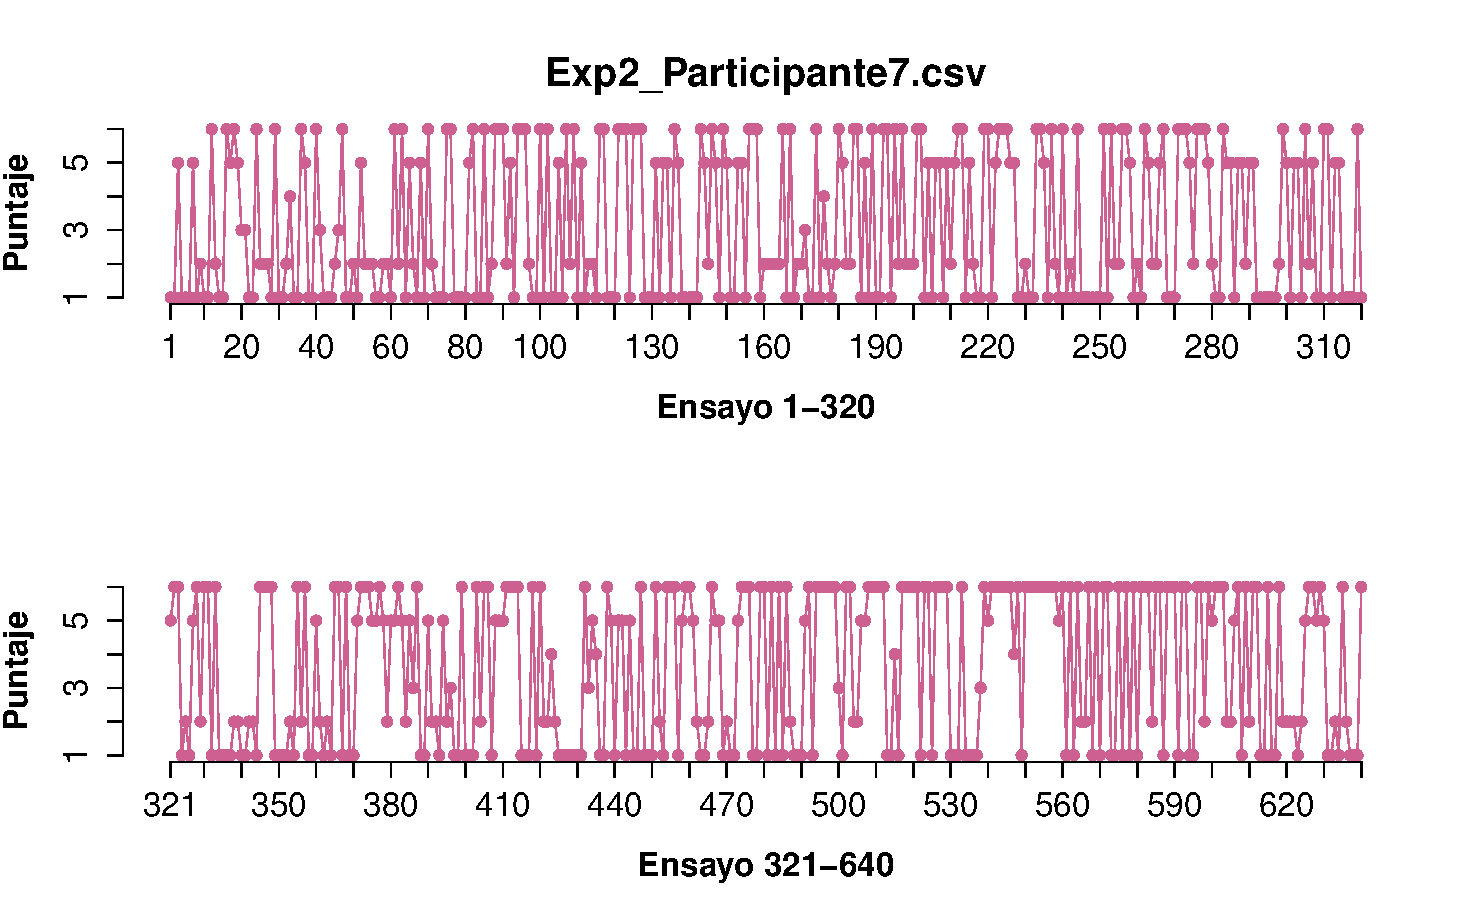
\includegraphics[width=0.30\textwidth]{Figures/Rating_Exp2_P7} 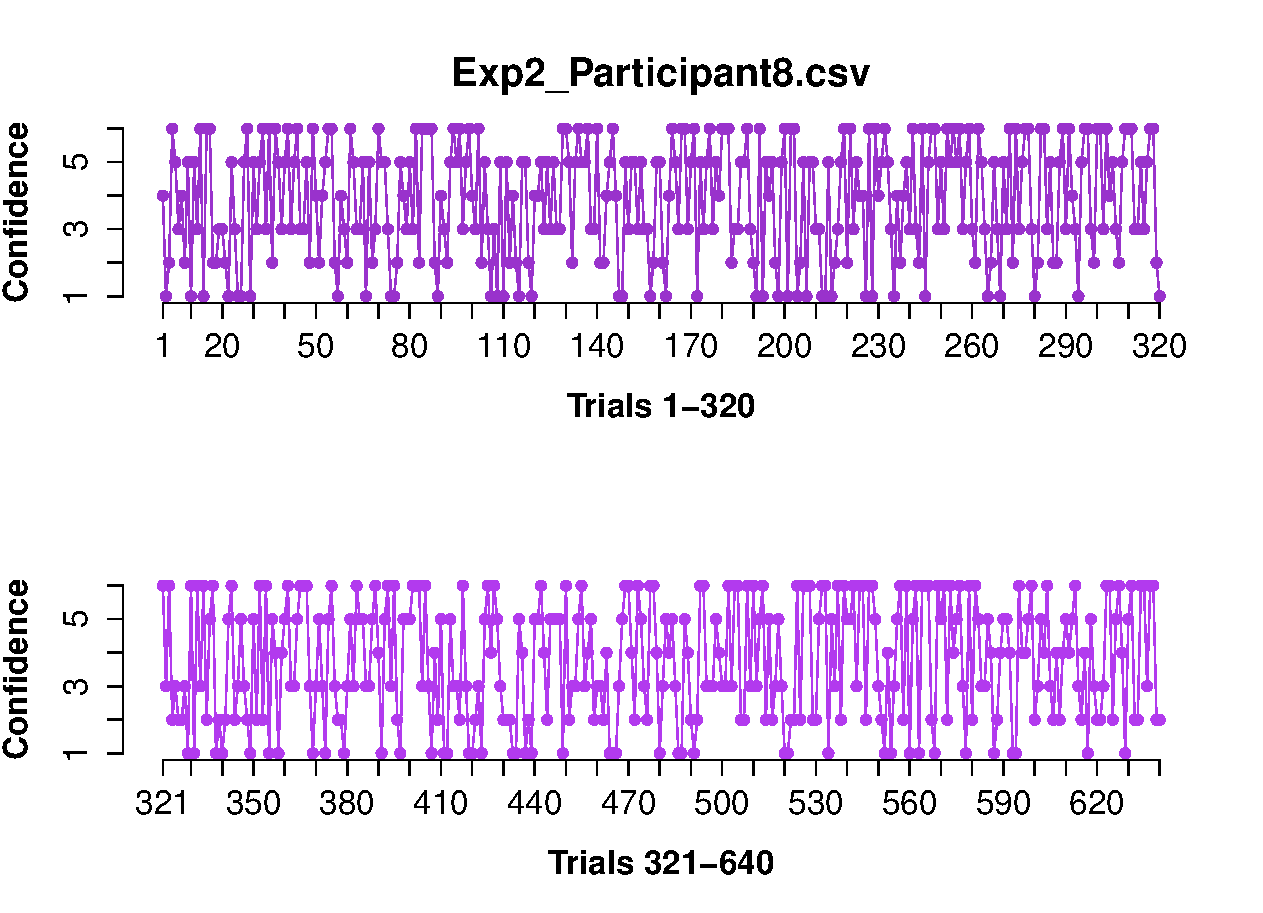
\includegraphics[width=0.30\textwidth]{Figures/Rating_Exp2_P8} 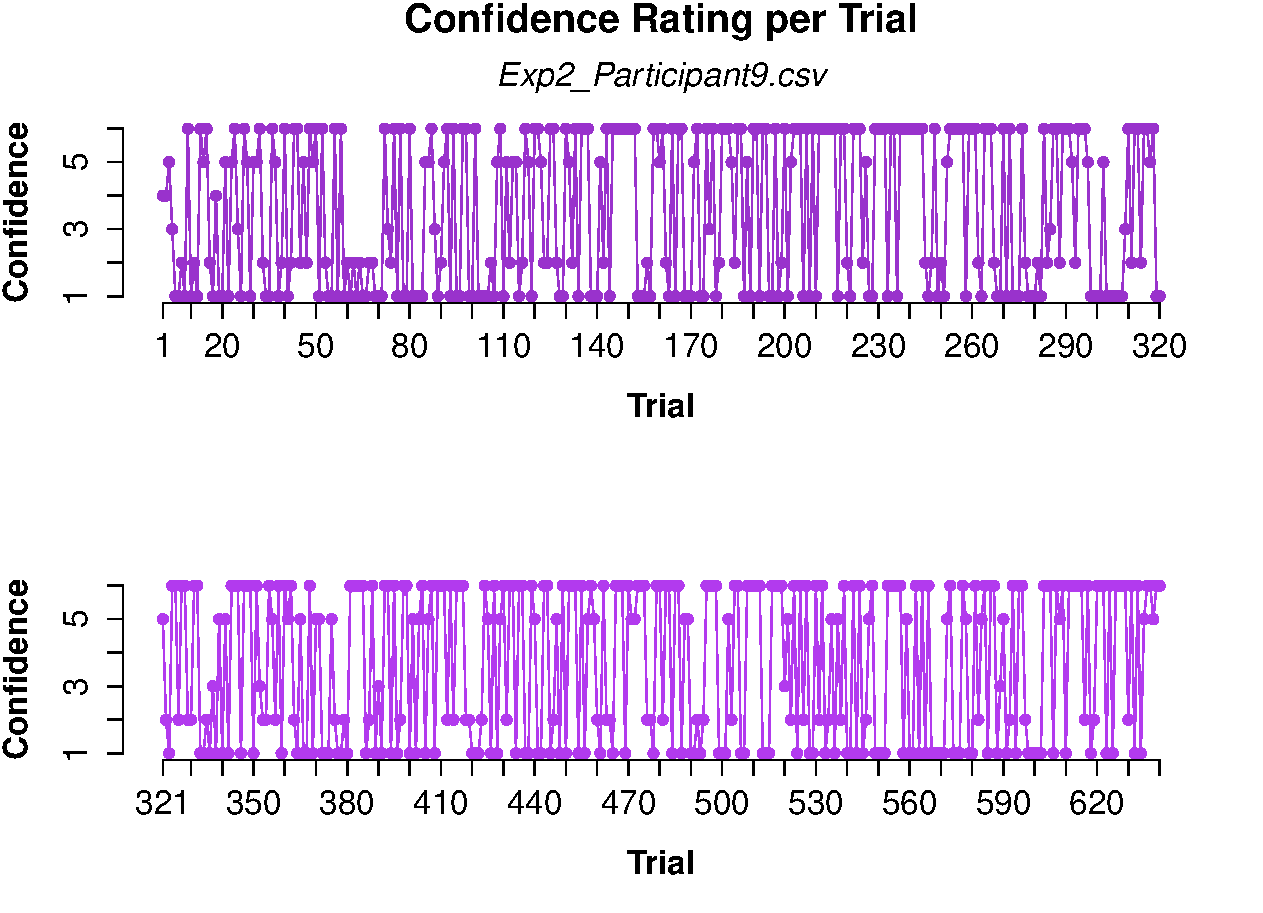
\includegraphics[width=0.30\textwidth]{Figures/Rating_Exp2_P9}
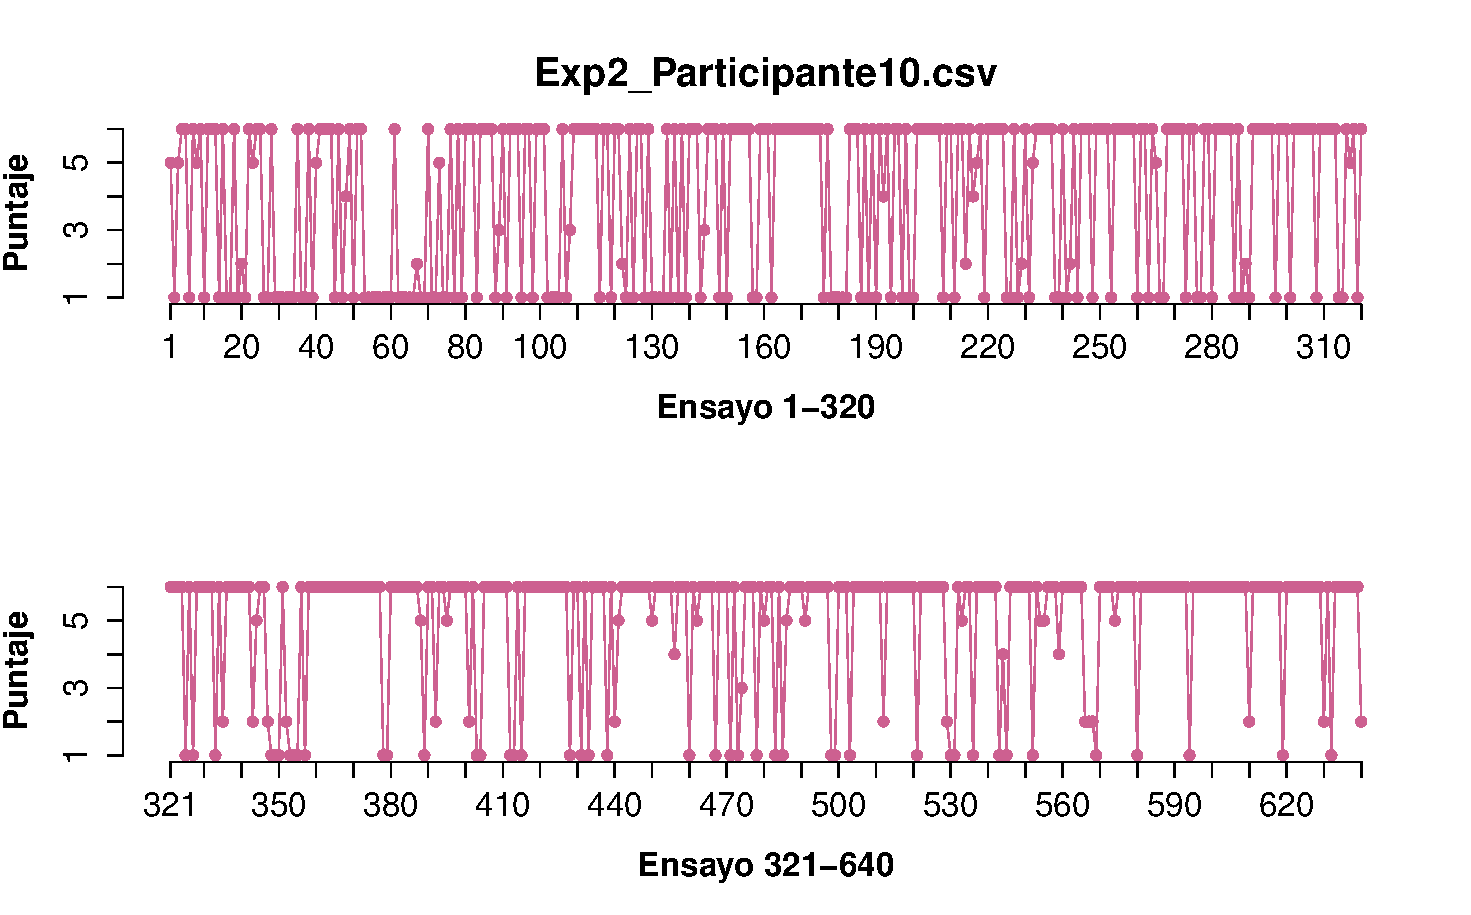
\includegraphics[width=0.30\textwidth]{Figures/Rating_Exp2_P10} 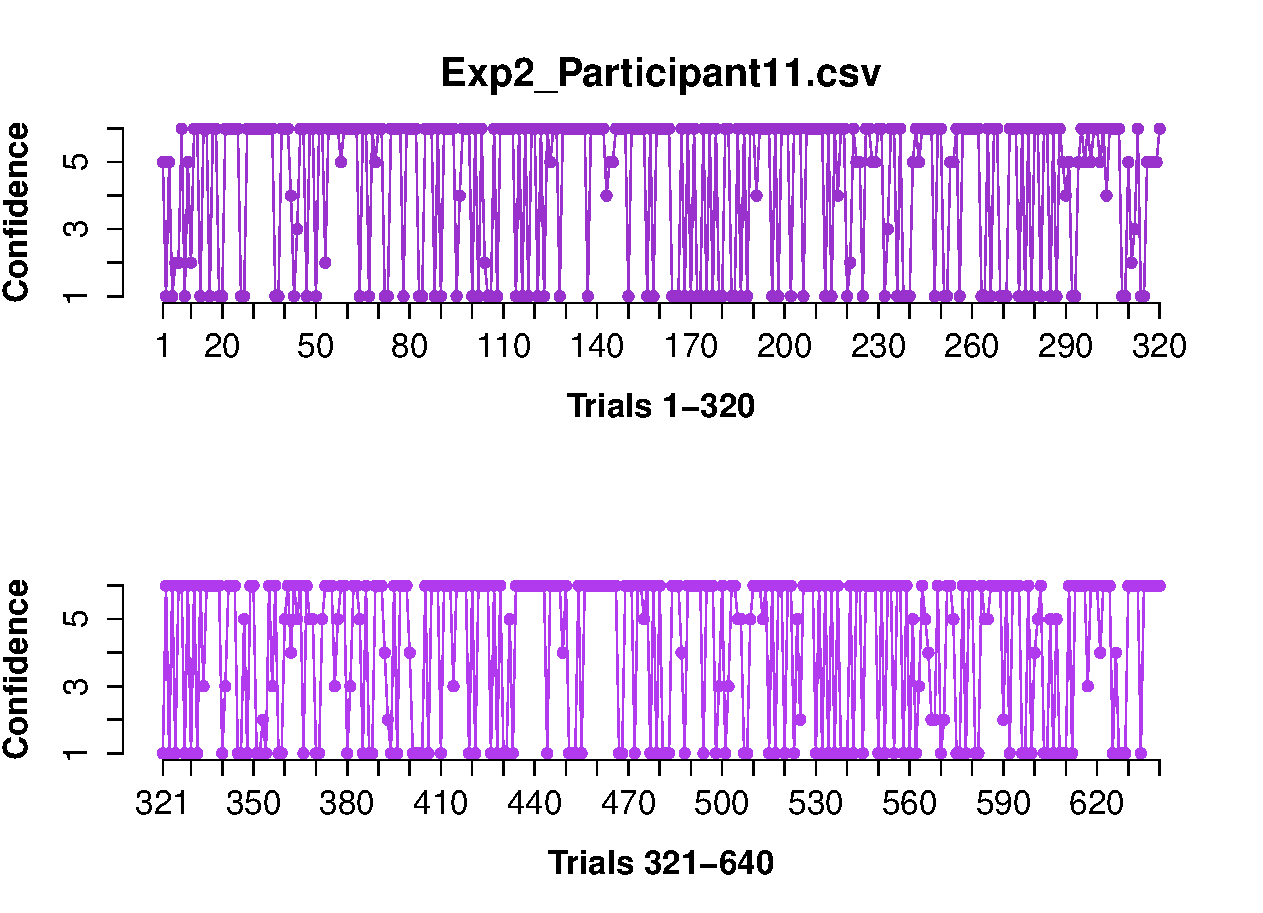
\includegraphics[width=0.30\textwidth]{Figures/Rating_Exp2_P11} 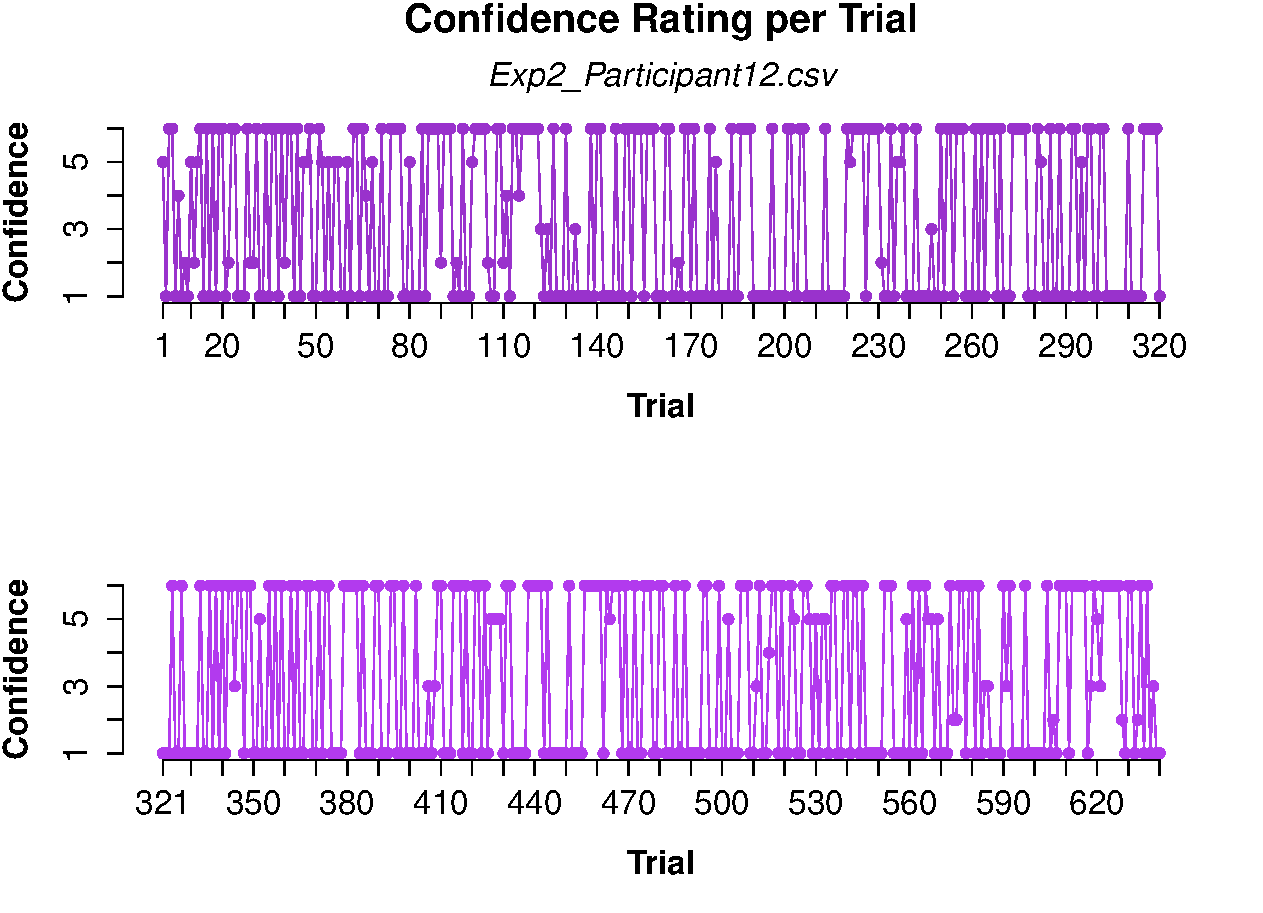
\includegraphics[width=0.30\textwidth]{Figures/Rating_Exp2_P12}
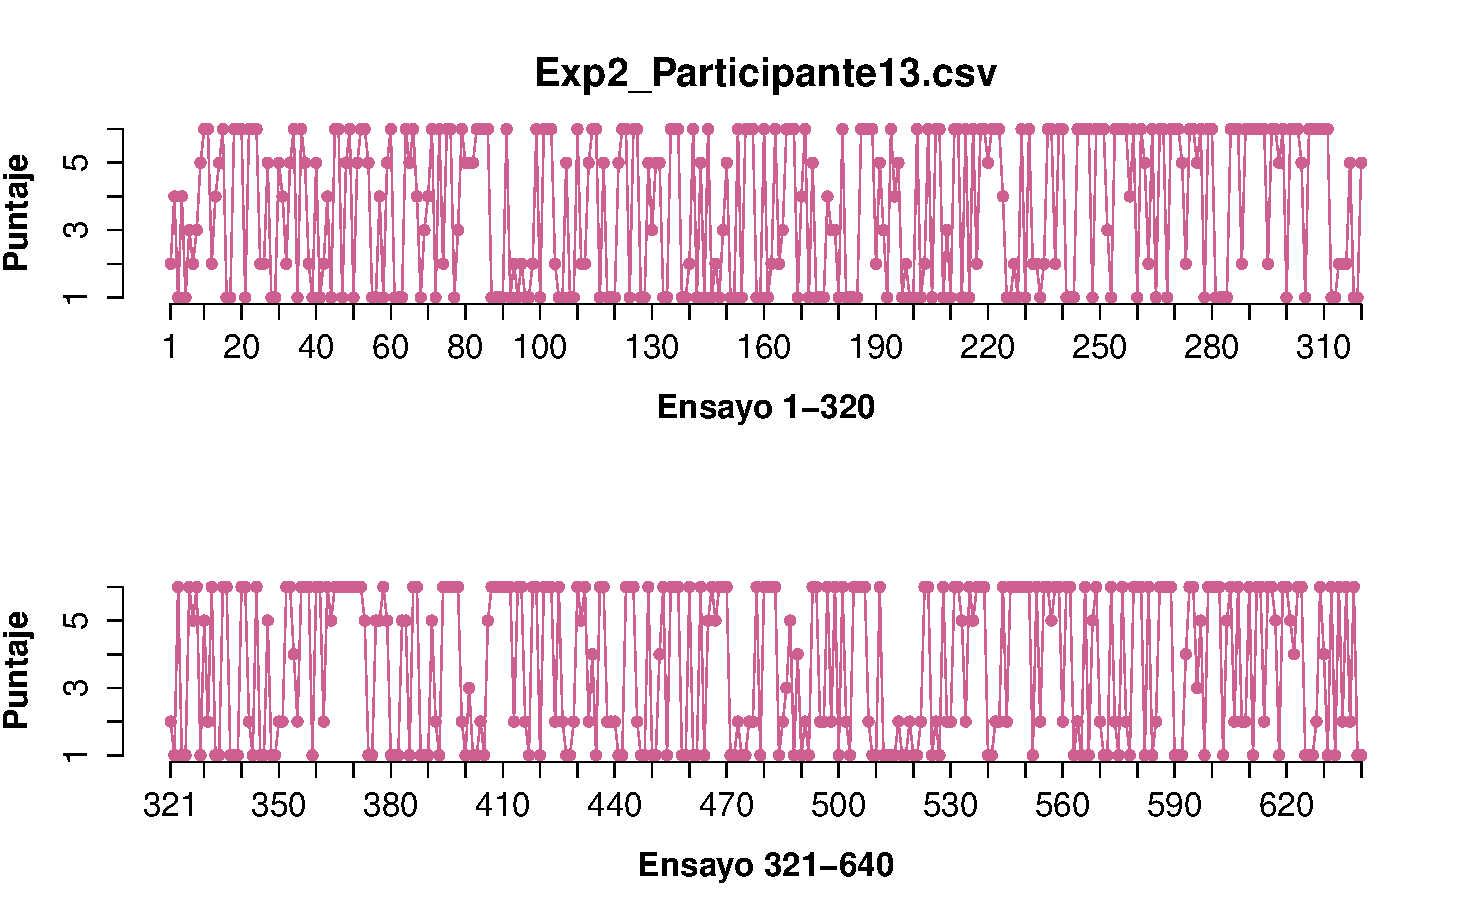
\includegraphics[width=0.30\textwidth]{Figures/Rating_Exp2_P13} 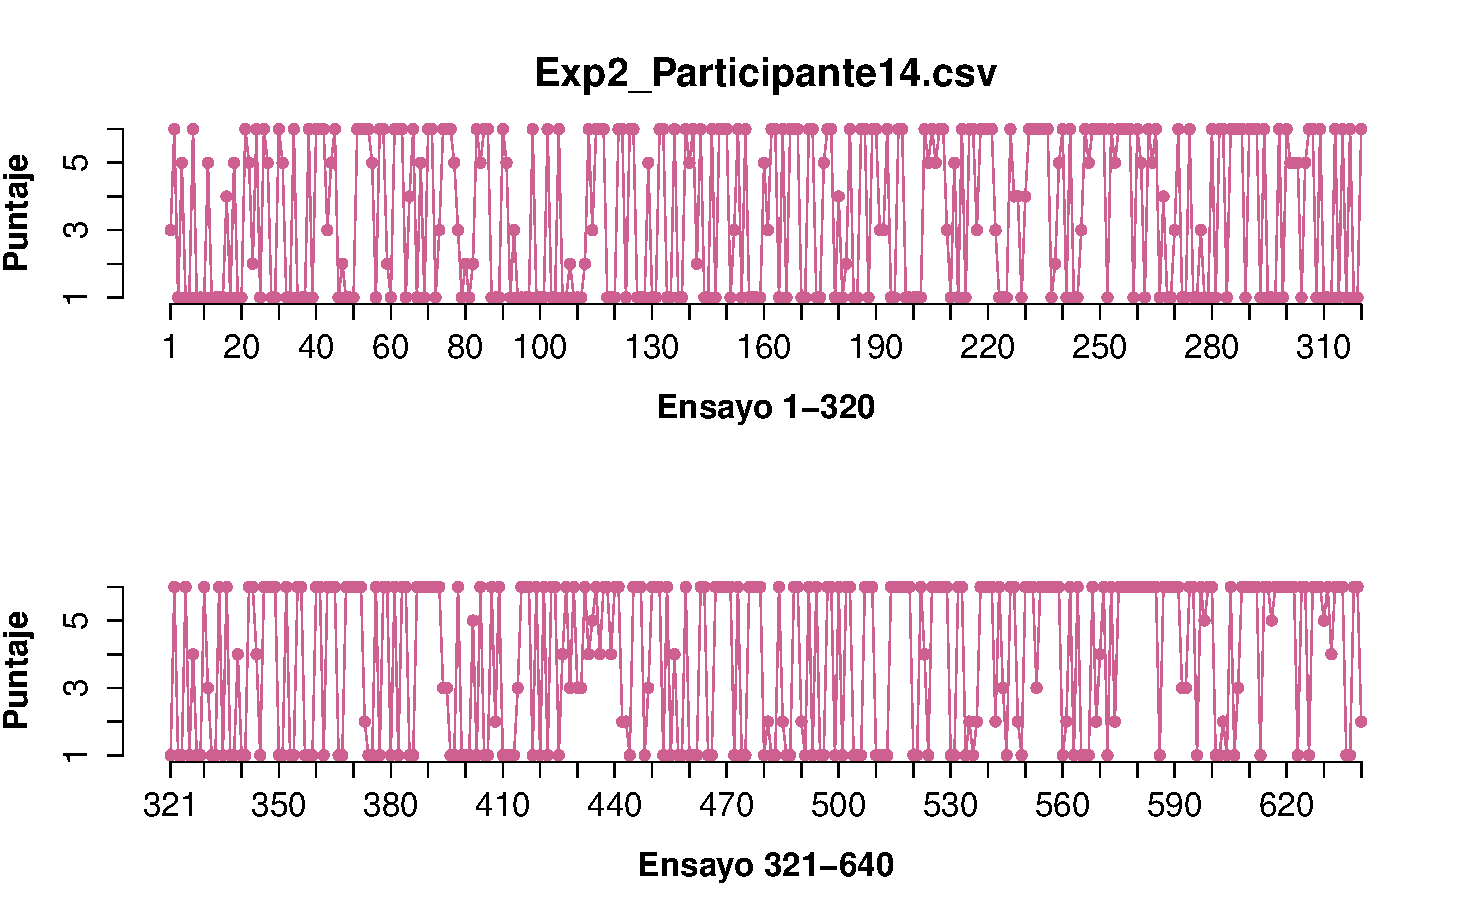
\includegraphics[width=0.30\textwidth]{Figures/Rating_Exp2_P14} 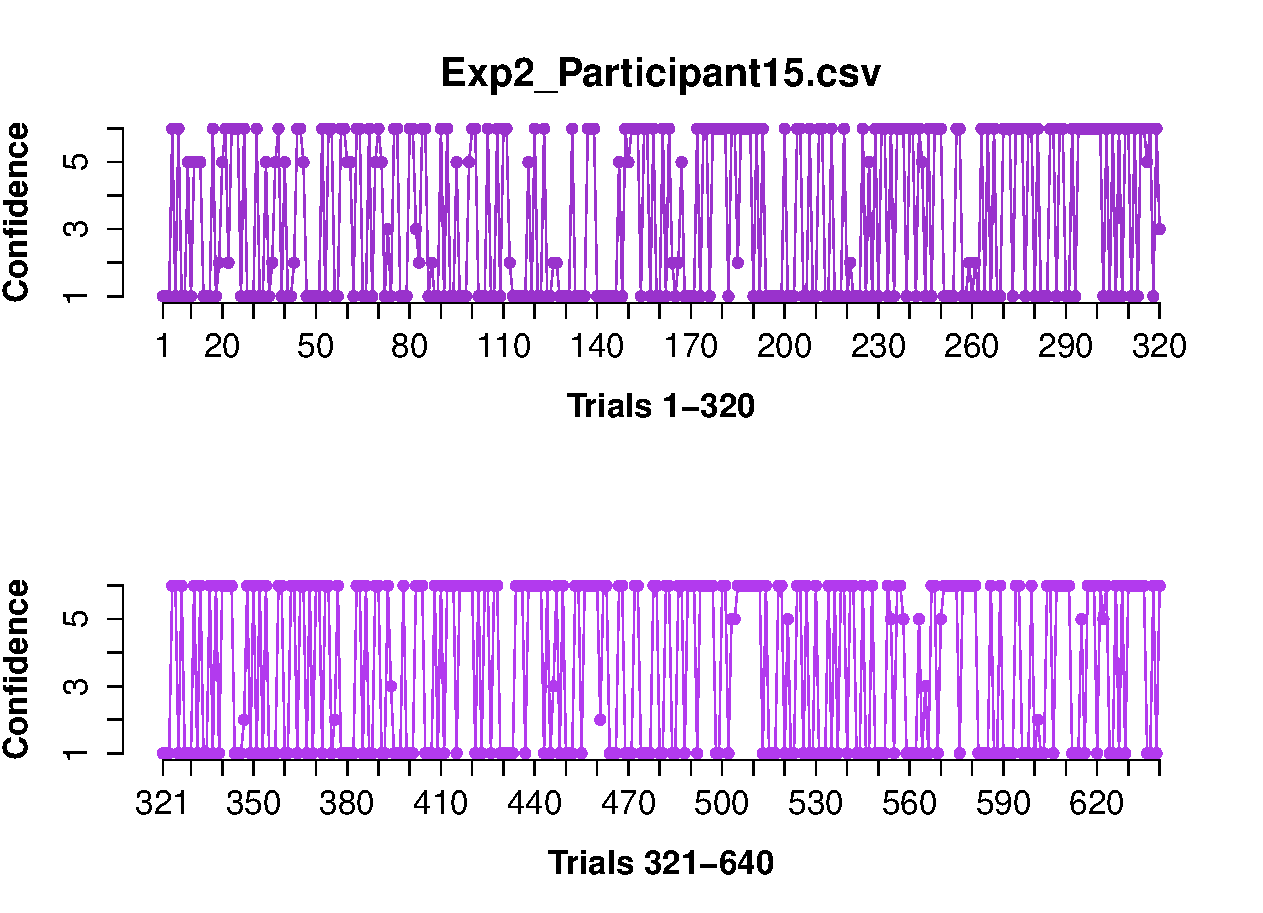
\includegraphics[width=0.30\textwidth]{Figures/Rating_Exp2_P15}
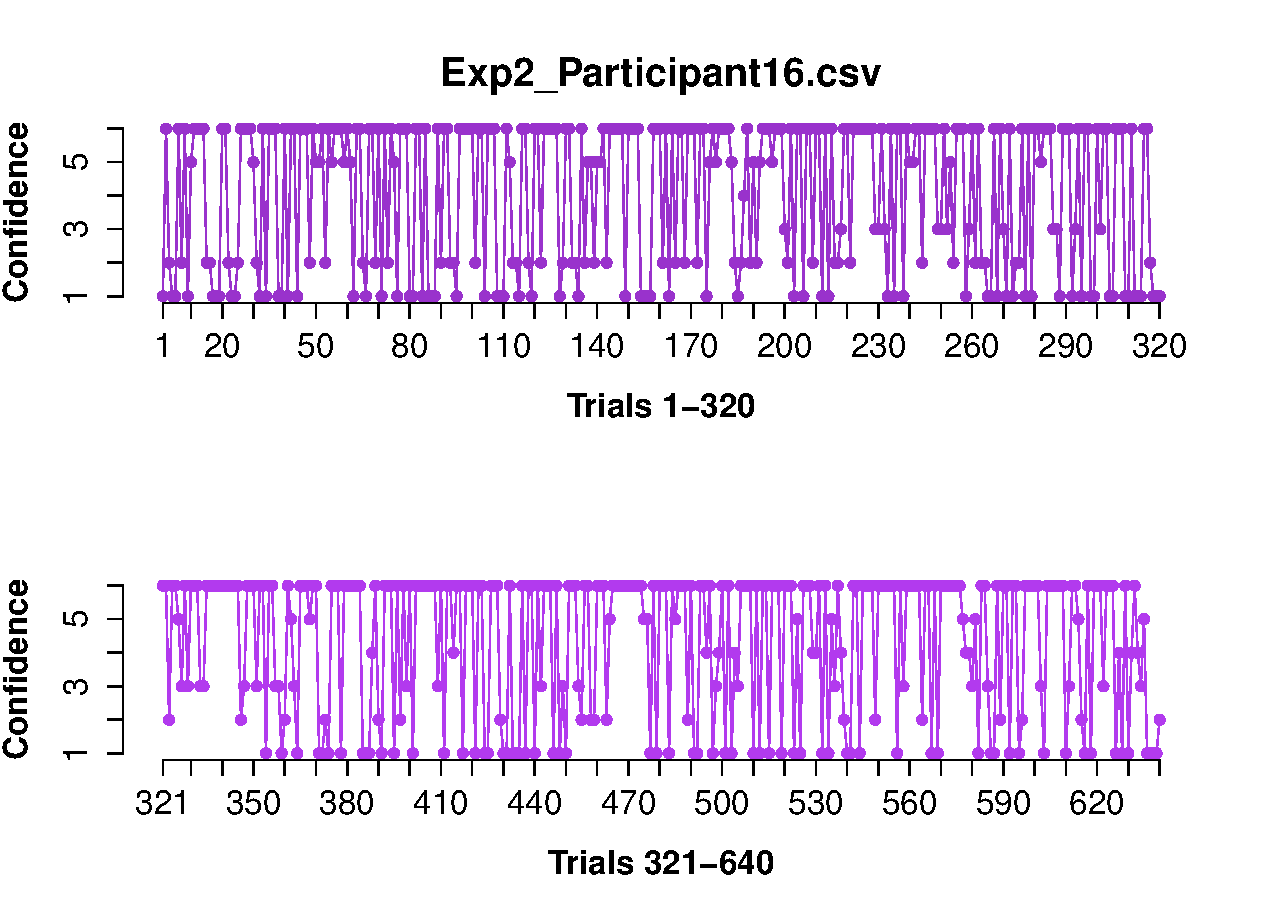
\includegraphics[width=0.30\textwidth]{Figures/Rating_Exp2_P16} 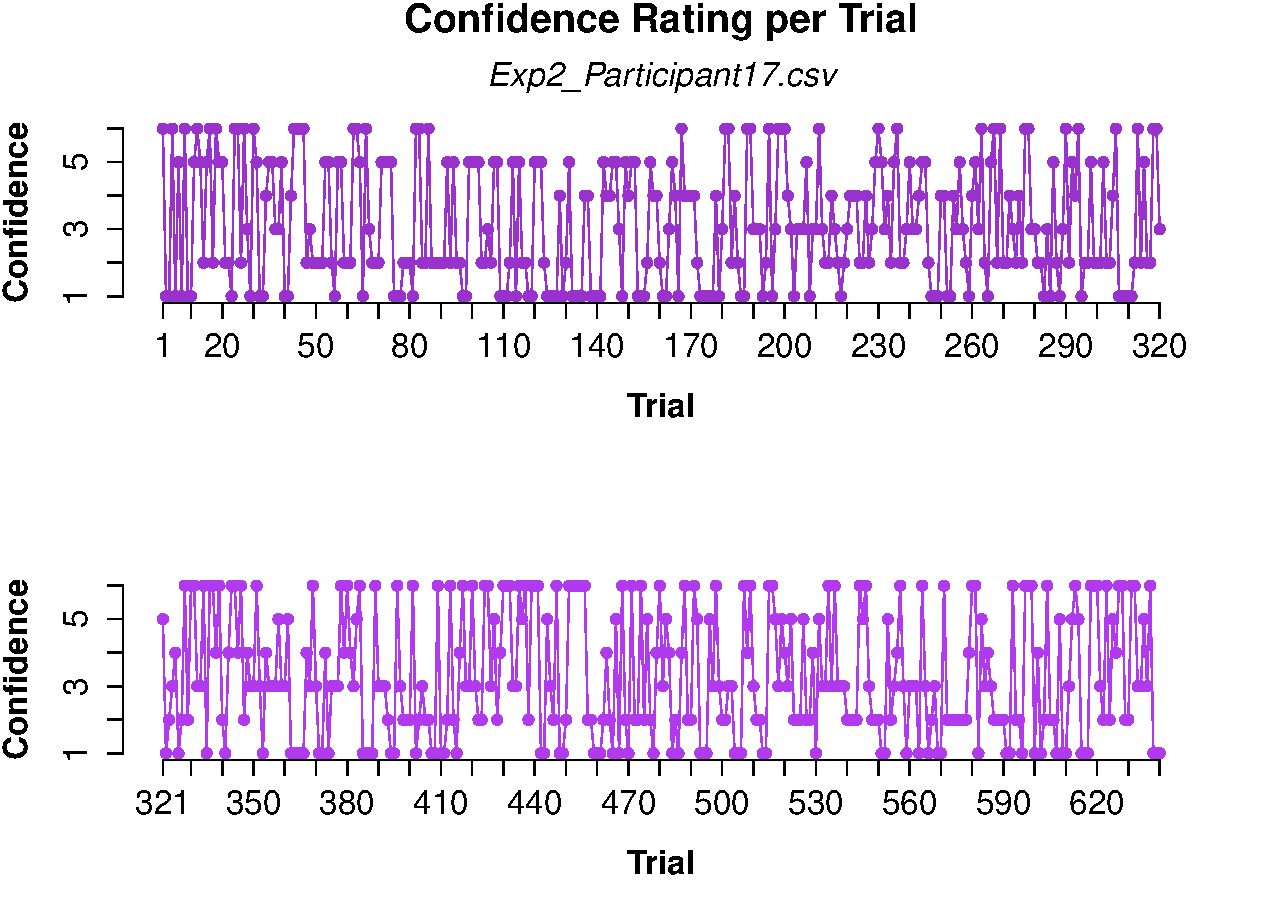
\includegraphics[width=0.30\textwidth]{Figures/Rating_Exp2_P17} 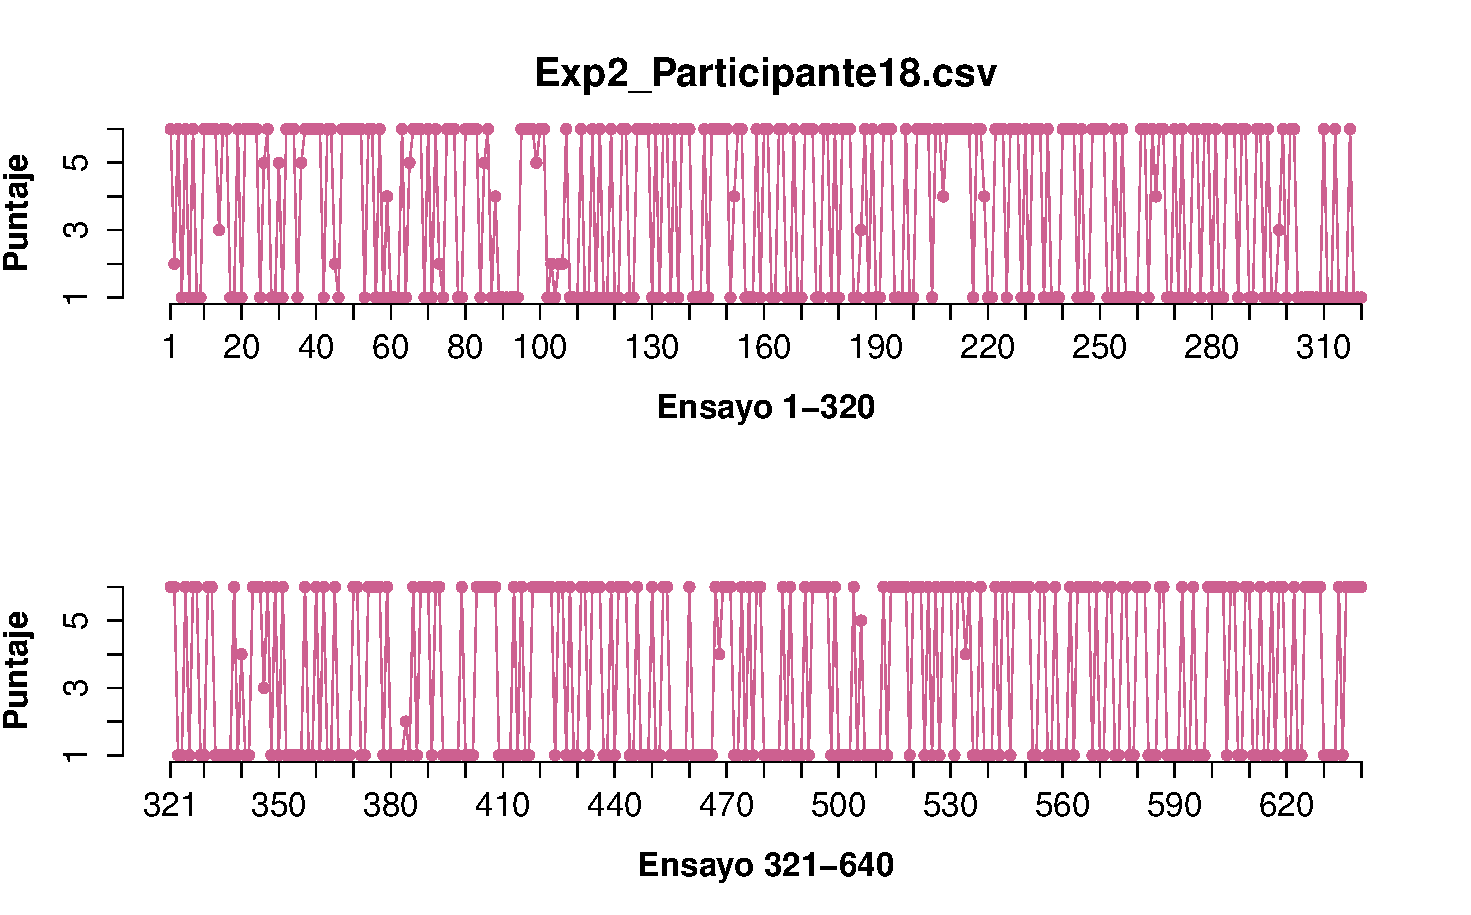
\includegraphics[width=0.30\textwidth]{Figures/Rating_Exp2_P18}
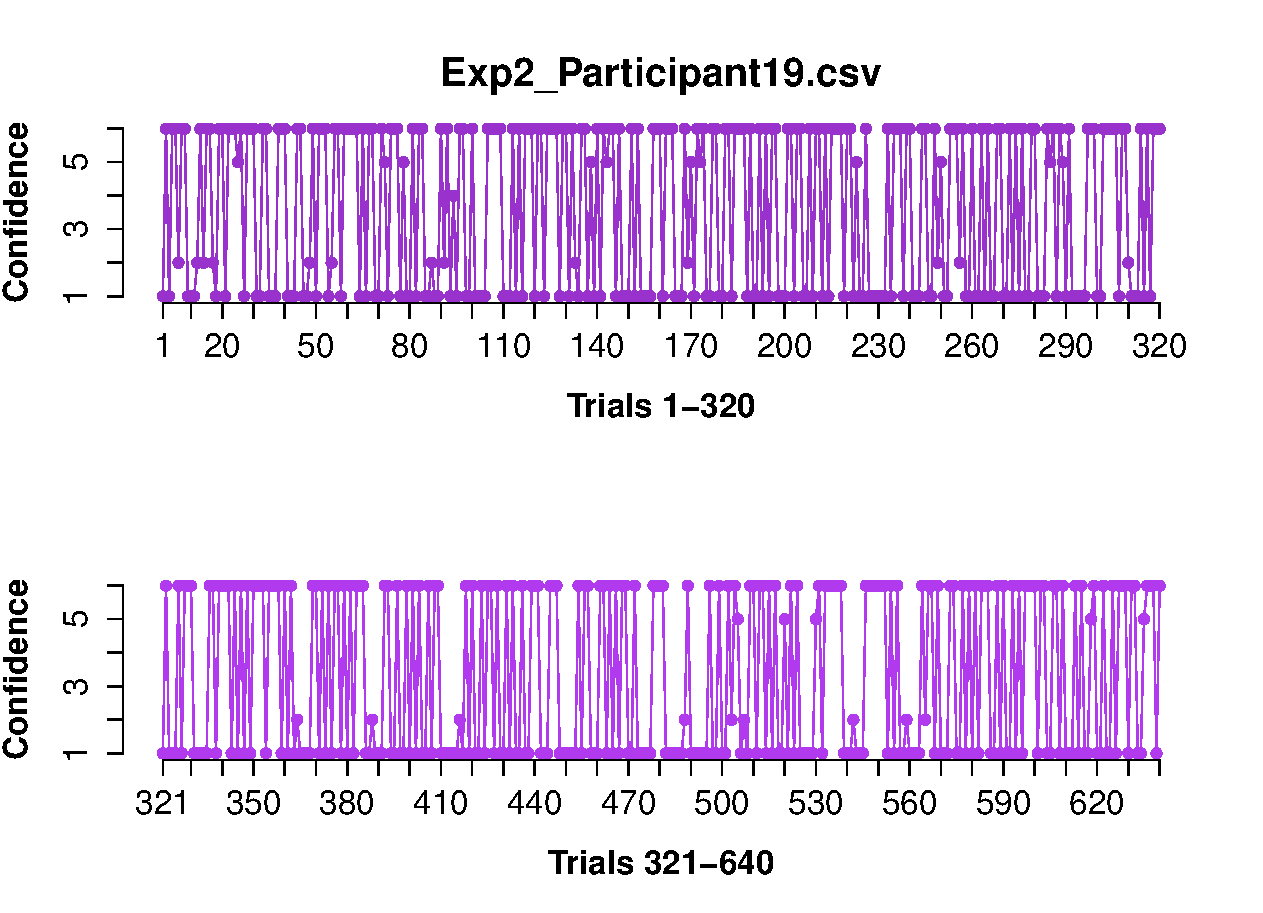
\includegraphics[width=0.30\textwidth]{Figures/Rating_Exp2_P19} 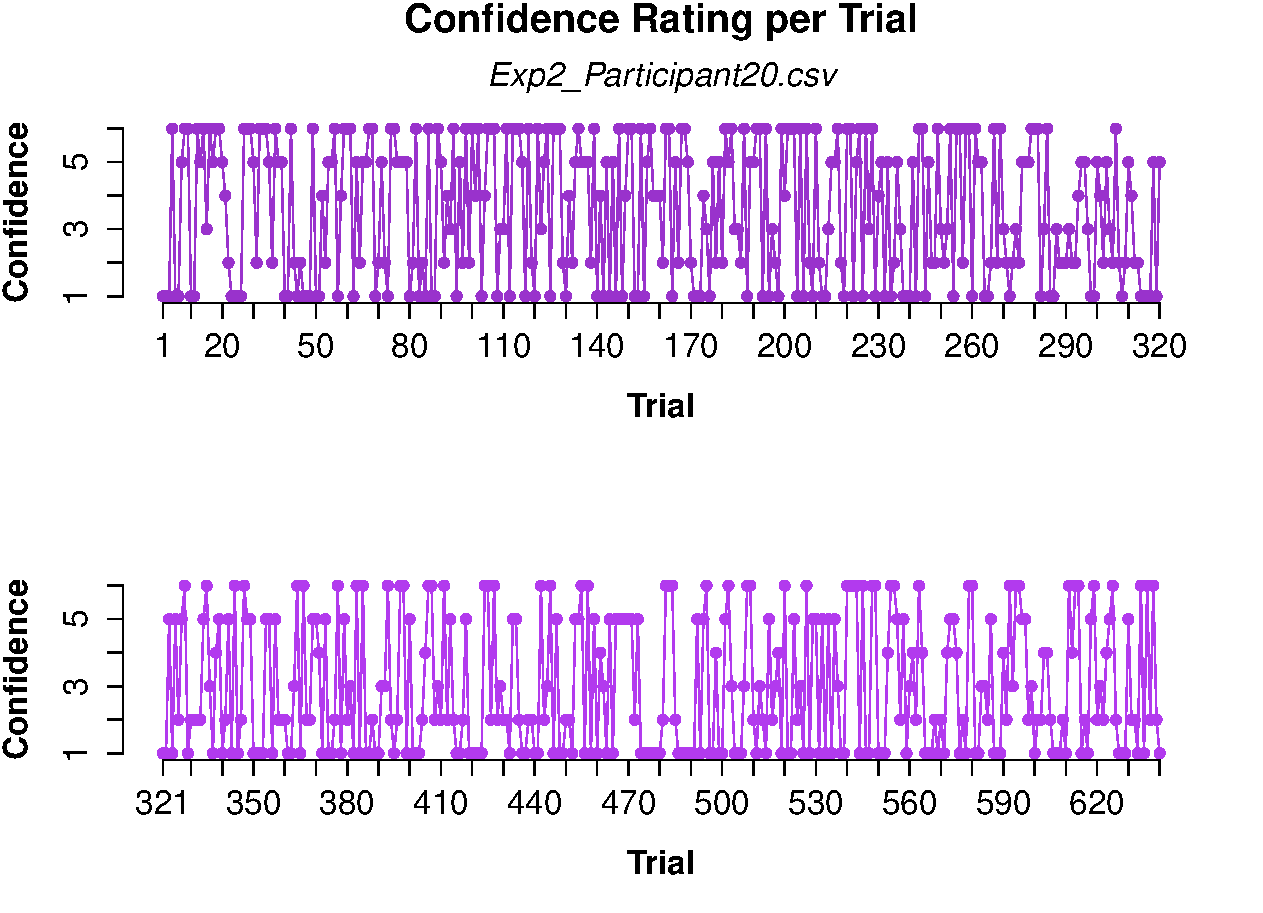
\includegraphics[width=0.30\textwidth]{Figures/Rating_Exp2_P20} 
%\decoRule
\caption[Rating_Exp2]{Escala por ensayo (Experimento 2).}
\label{fig:Rating_E2}
\end{figure}




\subsection{Control 2: Evaluando tiempos de respuesta a lo largo del experimento}


%%%%%%%%%%%%%%%%%%%%%%%%%%%%%%%%%%%%%%%%%%%%%%%%%%%%%%%%%%%%%%
%%%%%%%%%  Respuesta Rating en los ensayos
% Experimento 2
%%%%%%%%%%%%%%%%%%%%%%%%%%%%%%%%%%%%%%%%%%%%%%%%%%%%%%%%%%%%%%%
\begin{figure}[th]
\centering
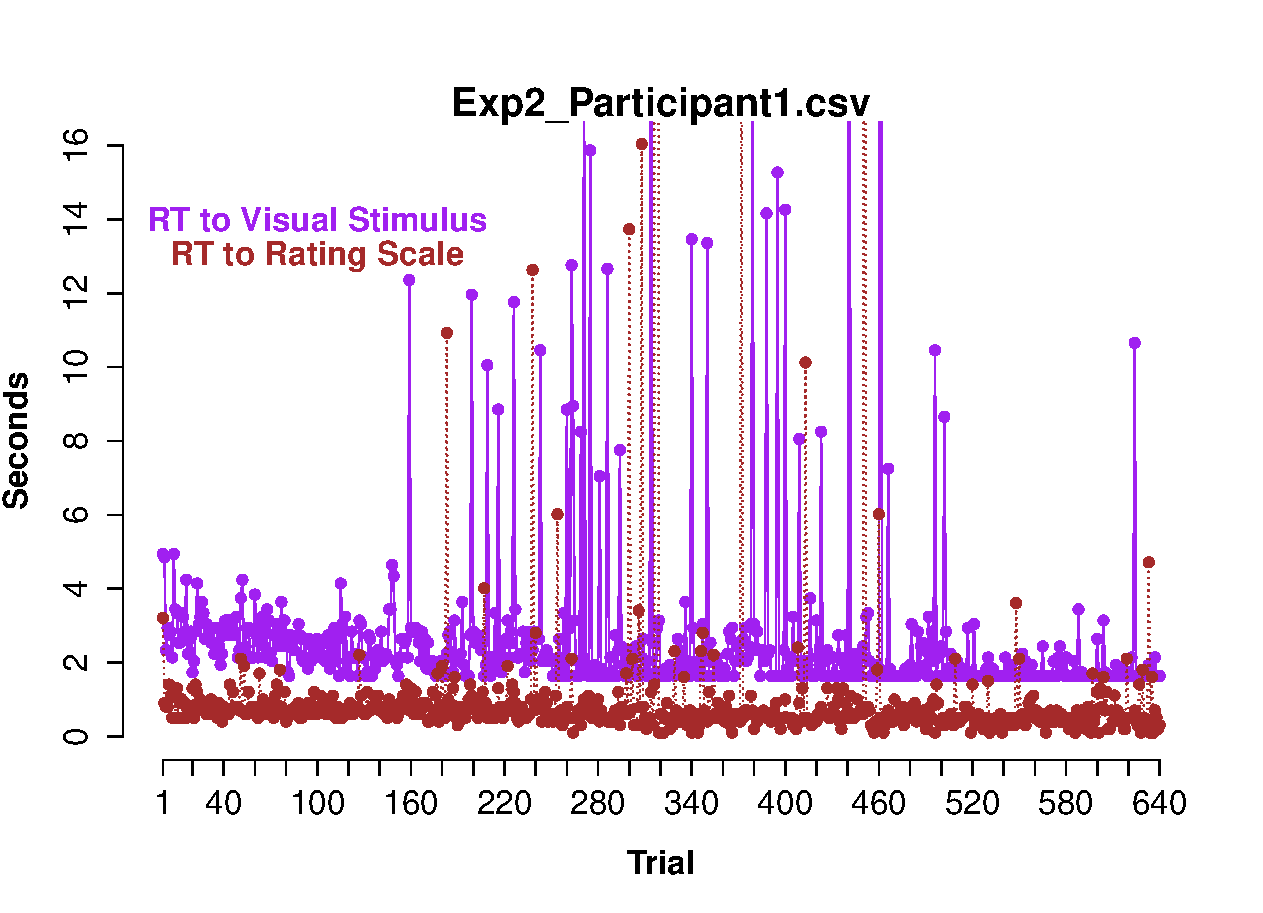
\includegraphics[width=0.30\textwidth]{Figures/RTs_Exp2_P1} 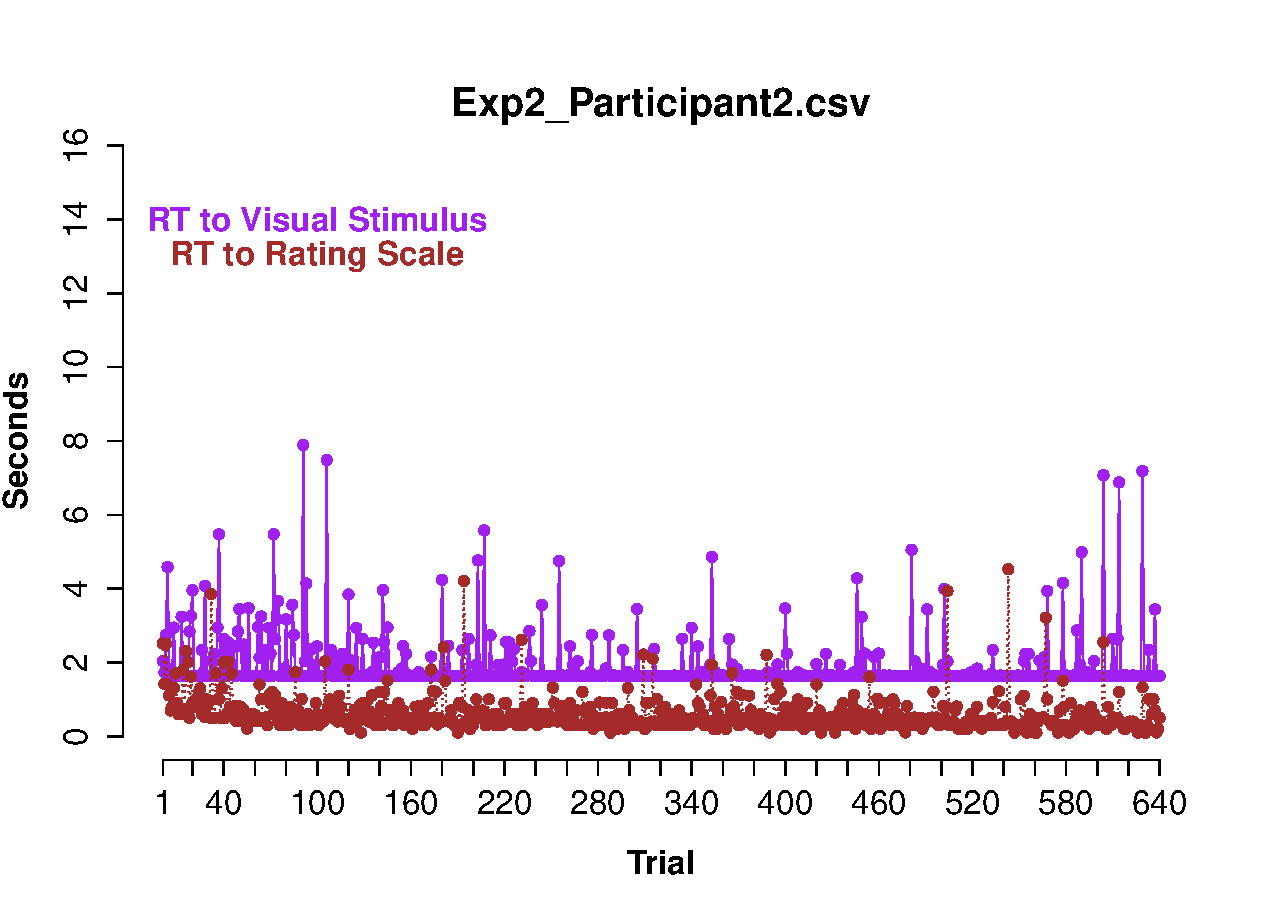
\includegraphics[width=0.30\textwidth]{Figures/RTs_Exp2_P2} 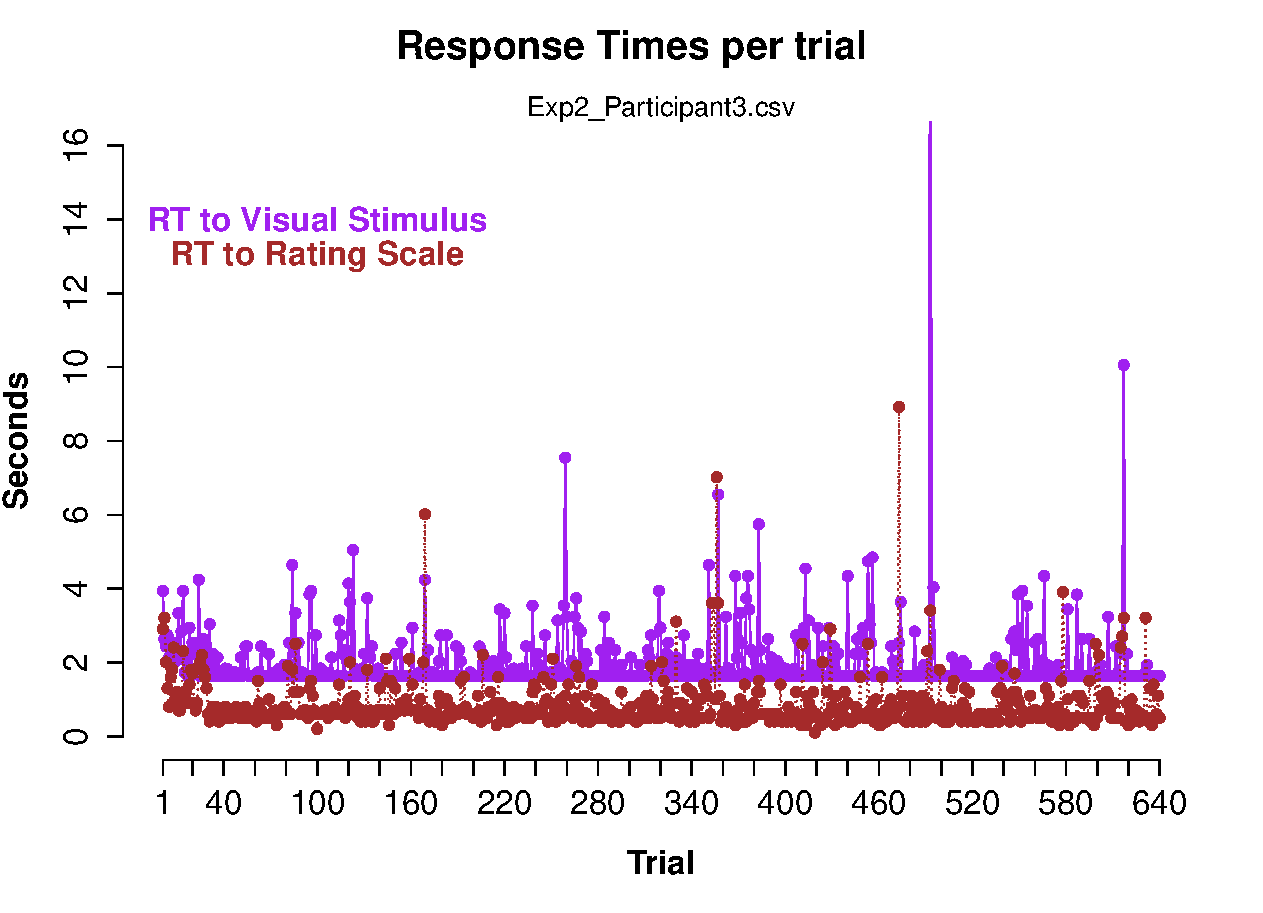
\includegraphics[width=0.30\textwidth]{Figures/RTs_Exp2_P3}
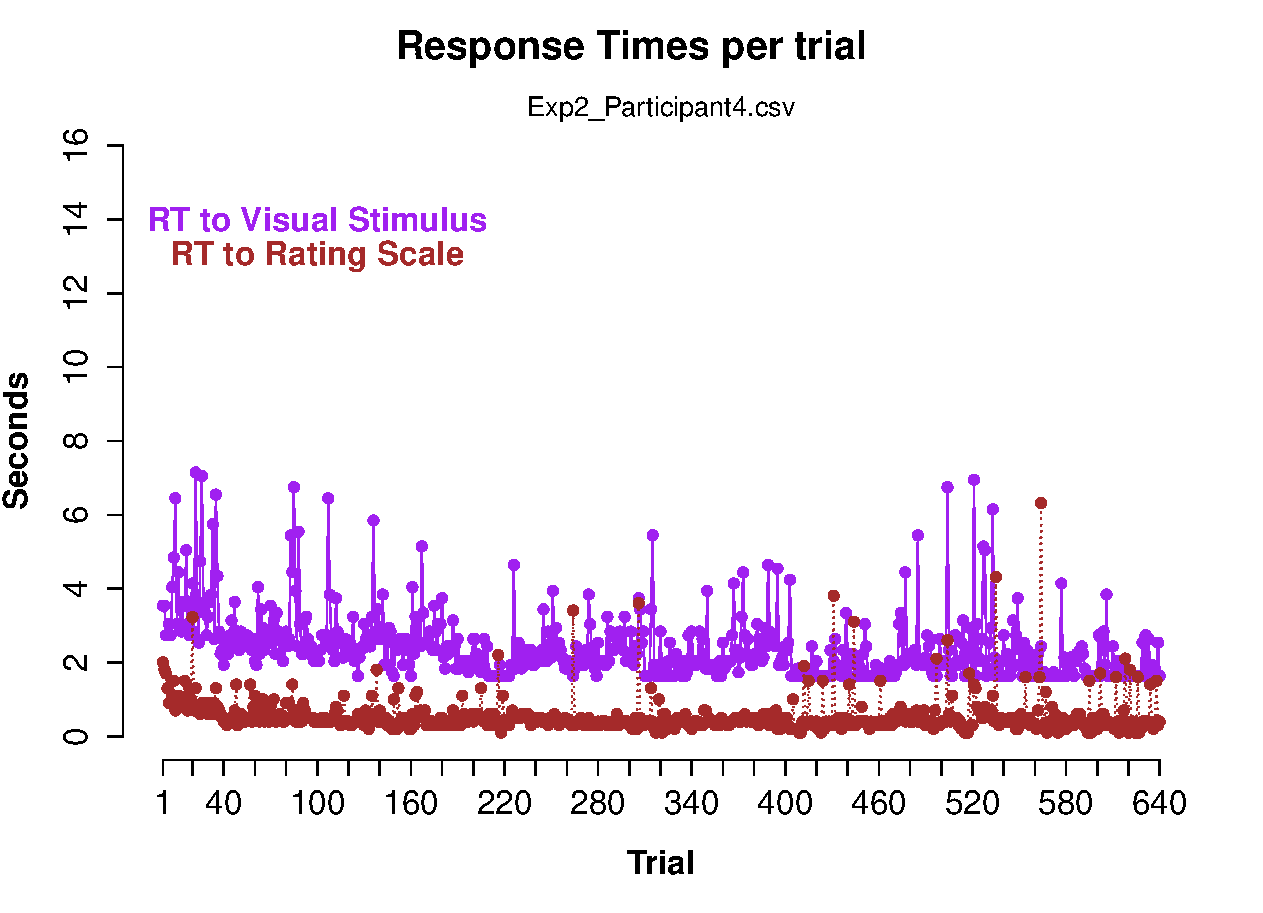
\includegraphics[width=0.30\textwidth]{Figures/RTs_Exp2_P4} 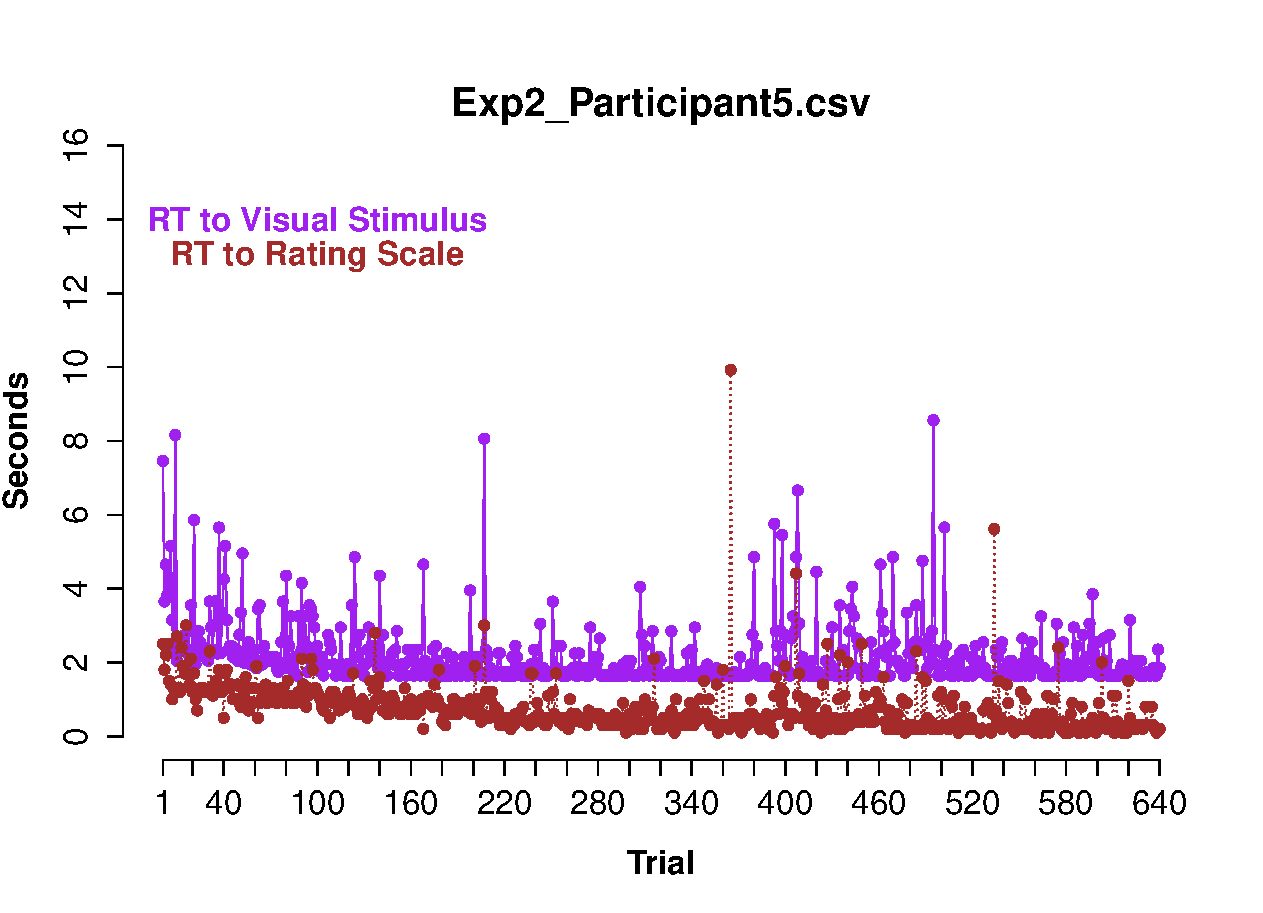
\includegraphics[width=0.30\textwidth]{Figures/RTs_Exp2_P5} 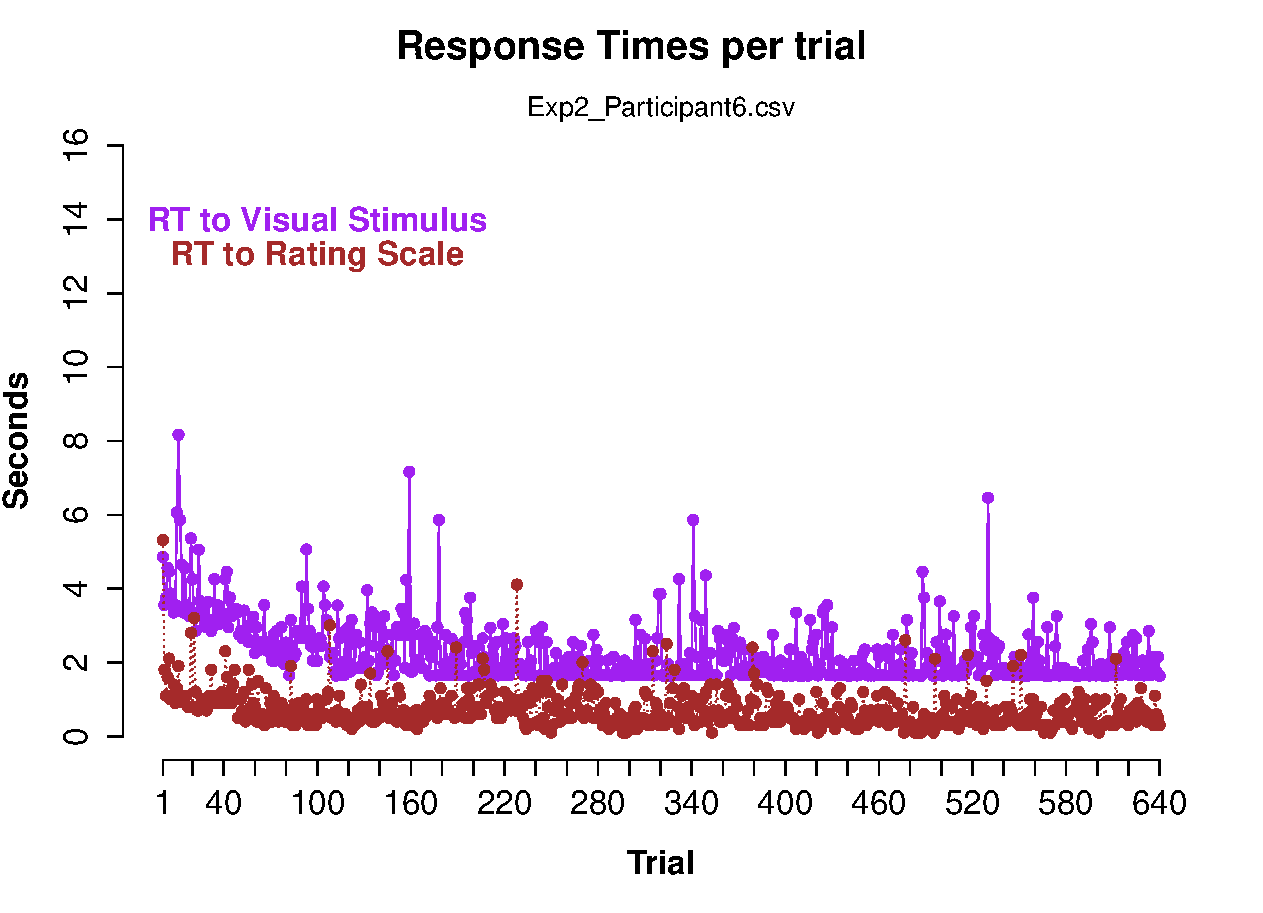
\includegraphics[width=0.30\textwidth]{Figures/RTs_Exp2_P6}
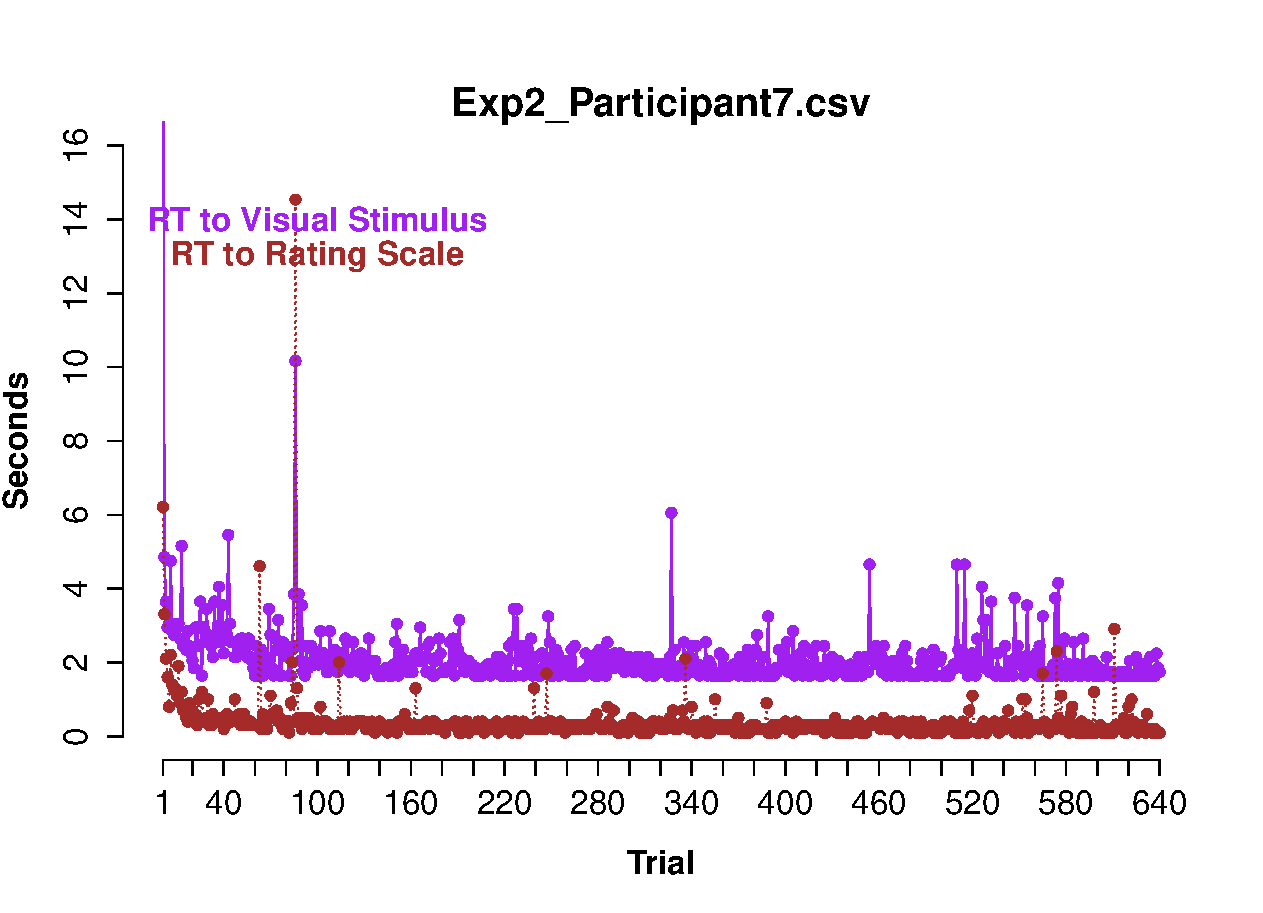
\includegraphics[width=0.30\textwidth]{Figures/RTs_Exp2_P7} 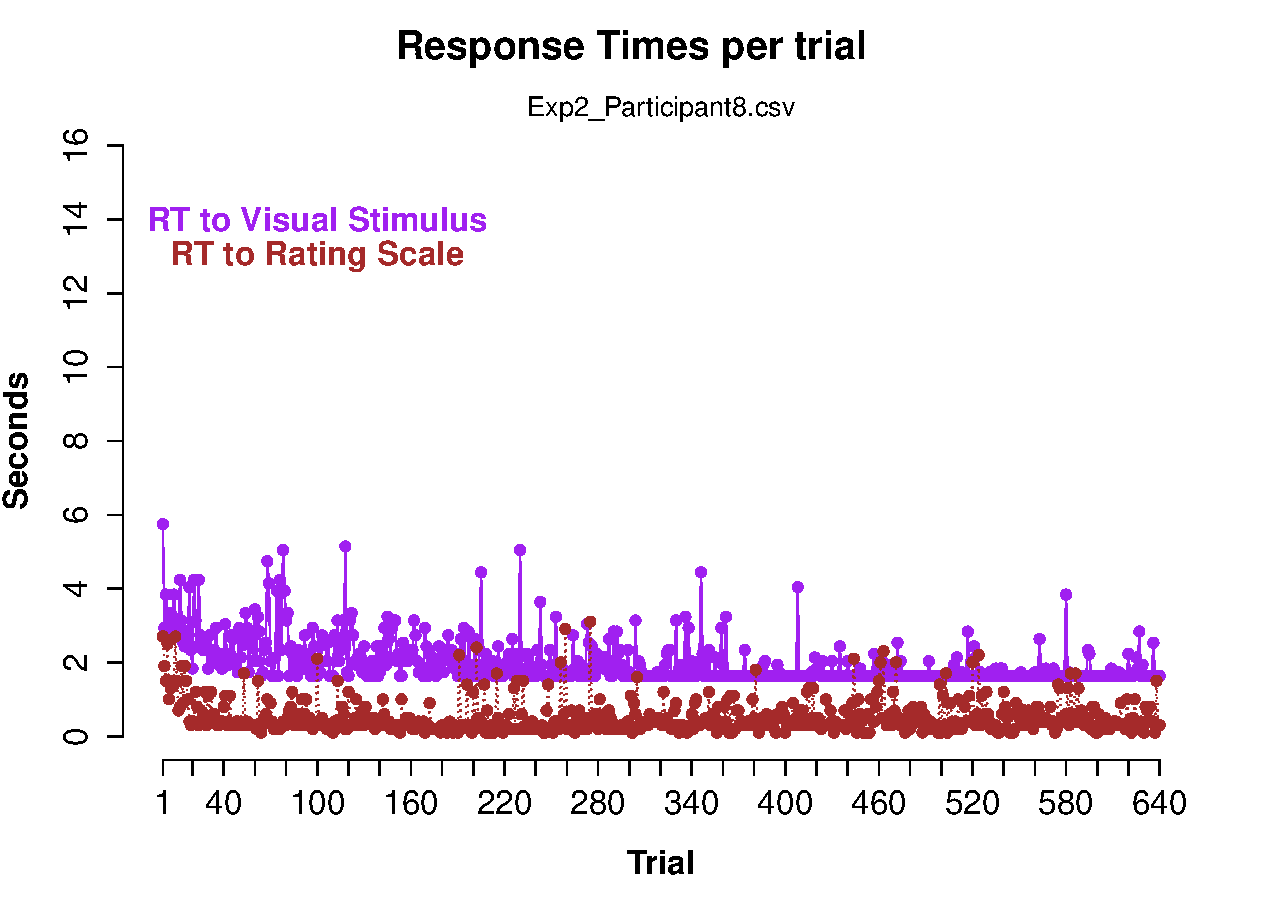
\includegraphics[width=0.30\textwidth]{Figures/RTs_Exp2_P8} 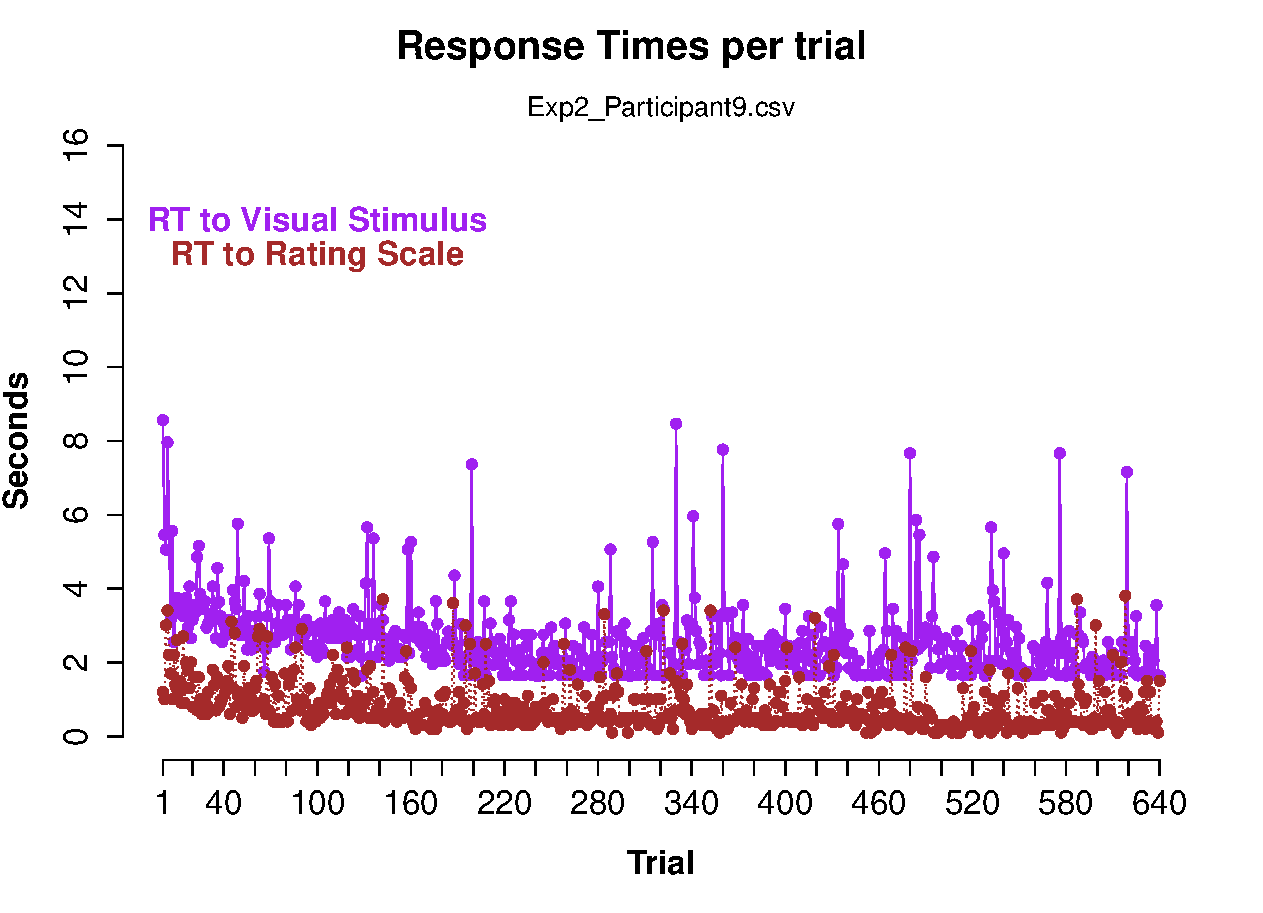
\includegraphics[width=0.30\textwidth]{Figures/RTs_Exp2_P9}
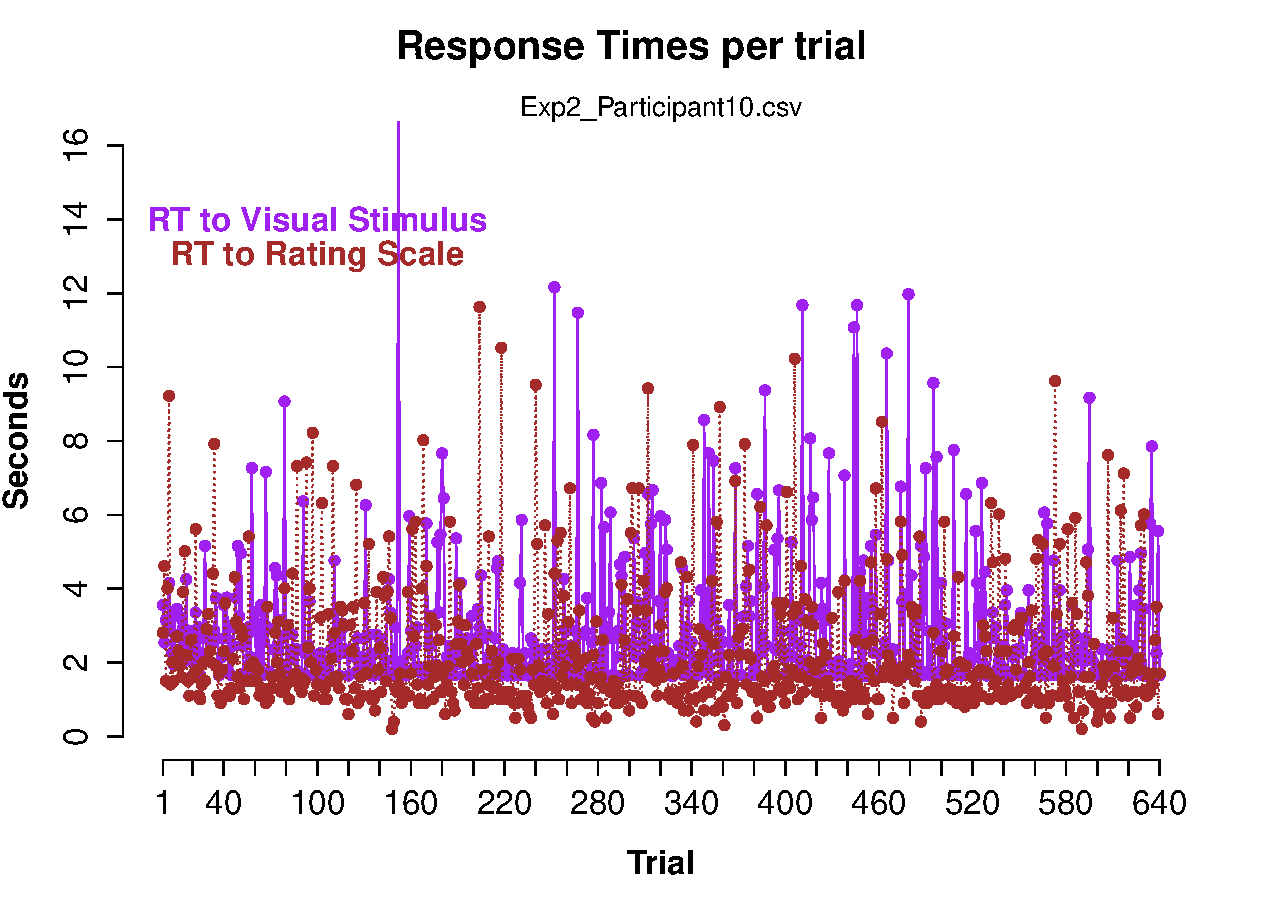
\includegraphics[width=0.30\textwidth]{Figures/RTs_Exp2_P10} \includegraphics[width=0.30\textwidth]{Figures/RTs_Exp2_P11} \includegraphics[width=0.30\textwidth]{Figures/RTs_Exp2_P12}
\includegraphics[width=0.30\textwidth]{Figures/RTs_Exp2_P13} \includegraphics[width=0.30\textwidth]{Figures/RTs_Exp2_P14} \includegraphics[width=0.30\textwidth]{Figures/RTs_Exp2_P15}
\includegraphics[width=0.30\textwidth]{Figures/RTs_Exp2_P16} \includegraphics[width=0.30\textwidth]{Figures/RTs_Exp2_P17} \includegraphics[width=0.30\textwidth]{Figures/RTs_Exp2_P18}
\includegraphics[width=0.30\textwidth]{Figures/RTs_Exp2_P19} \includegraphics[width=0.30\textwidth]{Figures/RTs_Exp2_P20} 
%\decoRule
\caption[Rating_Exp2]{Escala por ensayo (Experimento 2).}
\label{fig:Rating_E2}
\end{figure}


%%%%%%%%%%%%%%%%%%%%%%%%%%%%%%%%%%%%%%%%%%%%%%%%%%%%%%%%%%%%%%
%%%%%%%%%  Respuesta Rating en los ensayos
% Experimento 2
%%%%%%%%%%%%%%%%%%%%%%%%%%%%%%%%%%%%%%%%%%%%%%%%%%%%%%%%%%%%%%%
\begin{figure}[th]
\centering
\includegraphics[width=0.30\textwidth]{Figures/RT1_Exp2_P1} \includegraphics[width=0.30\textwidth]{Figures/RT1_Exp2_P2} \includegraphics[width=0.30\textwidth]{Figures/RT1_Exp2_P3}
\includegraphics[width=0.30\textwidth]{Figures/RT1_Exp2_P4} \includegraphics[width=0.30\textwidth]{Figures/RT1_Exp2_P5} \includegraphics[width=0.30\textwidth]{Figures/RT1_Exp2_P6}
\includegraphics[width=0.30\textwidth]{Figures/RT1_Exp2_P7} \includegraphics[width=0.30\textwidth]{Figures/RT1_Exp2_P8} \includegraphics[width=0.30\textwidth]{Figures/RT1_Exp2_P9}
\includegraphics[width=0.30\textwidth]{Figures/RT1_Exp2_P10} \includegraphics[width=0.30\textwidth]{Figures/RT1_Exp2_P11} \includegraphics[width=0.30\textwidth]{Figures/RT1_Exp2_P12}
\includegraphics[width=0.30\textwidth]{Figures/RT1_Exp2_P13} \includegraphics[width=0.30\textwidth]{Figures/RT1_Exp2_P14} \includegraphics[width=0.30\textwidth]{Figures/RT1_Exp2_P15}
\includegraphics[width=0.30\textwidth]{Figures/RT1_Exp2_P16} \includegraphics[width=0.30\textwidth]{Figures/RT1_Exp2_P17} \includegraphics[width=0.30\textwidth]{Figures/RT1_Exp2_P18}
\includegraphics[width=0.30\textwidth]{Figures/RT1_Exp2_P19} \includegraphics[width=0.30\textwidth]{Figures/RT1_Exp2_P20} 
%\decoRule
\caption[Rating_Exp2]{Escala por ensayo (Experimento 2).}
\label{fig:Rating_E2}
\end{figure}


%%%%%%%%%%%%%%%%%%%%%%%%%%%%%%%%%%%%%%%%%%%%%%%%%%%%%%%%%%%%%%
%%%%%%%%%  Respuesta Rating en los ensayos
% Experimento 2
%%%%%%%%%%%%%%%%%%%%%%%%%%%%%%%%%%%%%%%%%%%%%%%%%%%%%%%%%%%%%%%
\begin{figure}[th]
\centering
\includegraphics[width=0.30\textwidth]{Figures/RT2_Exp2_P1} \includegraphics[width=0.30\textwidth]{Figures/RT2_Exp2_P2} \includegraphics[width=0.30\textwidth]{Figures/RT2_Exp2_P3}
\includegraphics[width=0.30\textwidth]{Figures/RT2_Exp2_P4} \includegraphics[width=0.30\textwidth]{Figures/RT2_Exp2_P5} \includegraphics[width=0.30\textwidth]{Figures/RT2_Exp2_P6}
\includegraphics[width=0.30\textwidth]{Figures/RT2_Exp2_P7} \includegraphics[width=0.30\textwidth]{Figures/RT2_Exp2_P8} \includegraphics[width=0.30\textwidth]{Figures/RT2_Exp2_P9}
\includegraphics[width=0.30\textwidth]{Figures/RT2_Exp2_P10} \includegraphics[width=0.30\textwidth]{Figures/RT2_Exp2_P11} \includegraphics[width=0.30\textwidth]{Figures/RT2_Exp2_P12}
\includegraphics[width=0.30\textwidth]{Figures/RT2_Exp2_P13} \includegraphics[width=0.30\textwidth]{Figures/RT2_Exp2_P14} \includegraphics[width=0.30\textwidth]{Figures/RT2_Exp2_P15}
\includegraphics[width=0.30\textwidth]{Figures/RT2_Exp2_P16} \includegraphics[width=0.30\textwidth]{Figures/RT2_Exp2_P17} \includegraphics[width=0.30\textwidth]{Figures/RT2_Exp2_P18}
\includegraphics[width=0.30\textwidth]{Figures/RT2_Exp2_P19} \includegraphics[width=0.30\textwidth]{Figures/RT2_Exp2_P20} 
%\decoRule
\caption[Rating_Exp2]{Escala por ensayo (Experimento 2).}
\label{fig:Rating_E2}
\end{figure}



\subsection{Control 3: ¿La duración del experimento tuvo un impacto en la ejecución de los participantes?}


%%%%%%%%%%%%%%%%%%%%%%%%%%%%%%%%%%%%%%%%%%%%%%%%%%%%%%%%%%%%%%
%%%%%%%%%  Respuesta (Y/N) en los ensayos
% Experimento 2
%%%%%%%%%%%%%%%%%%%%%%%%%%%%%%%%%%%%%%%%%%%%%%%%%%%%%%%%%%%%%%%
\begin{figure}[th]
\centering
\includegraphics[width=0.30\textwidth]{Figures/Success_Exp2_P1} \includegraphics[width=0.30\textwidth]{Figures/Success_Exp2_P2} \includegraphics[width=0.30\textwidth]{Figures/Success_Exp2_P3}
\includegraphics[width=0.30\textwidth]{Figures/Success_Exp2_P4} \includegraphics[width=0.30\textwidth]{Figures/Success_Exp2_P5} \includegraphics[width=0.30\textwidth]{Figures/Success_Exp2_P6}
\includegraphics[width=0.30\textwidth]{Figures/Success_Exp2_P7} \includegraphics[width=0.30\textwidth]{Figures/Success_Exp2_P8} \includegraphics[width=0.30\textwidth]{Figures/Success_Exp2_P9}
\includegraphics[width=0.30\textwidth]{Figures/Success_Exp2_P10} \includegraphics[width=0.30\textwidth]{Figures/Success_Exp2_P11} \includegraphics[width=0.30\textwidth]{Figures/Success_Exp2_P12}
\includegraphics[width=0.30\textwidth]{Figures/Success_Exp2_P13} \includegraphics[width=0.30\textwidth]{Figures/Success_Exp2_P14} \includegraphics[width=0.30\textwidth]{Figures/Success_Exp2_P15}
\includegraphics[width=0.30\textwidth]{Figures/Success_Exp2_P16} \includegraphics[width=0.30\textwidth]{Figures/Success_Exp2_P17} \includegraphics[width=0.30\textwidth]{Figures/Success_Exp2_P18}
\includegraphics[width=0.30\textwidth]{Figures/Success_Exp2_P19} \includegraphics[width=0.30\textwidth]{Figures/Success_Exp2_P20} 
%\decoRule
\caption[Response_Exp2]{Respuesta por ensayo (Experimento 2).}
\label{fig:Response_E2}
\end{figure}


%%%%%%%%%%%%%%%%%%%%%%%%%%%%%%%%%%%%%%%%%%%%%%%%%%%%%%%%
%%%%%%%%%  Respuesta Rating en los ensayos
% Experimento 2
%%%%%%%%%%%%%%%%%%%%%%%%%%%%%%%%%%%%%%%%%%%%%%%%%%%%%%%%%%%%%%%
\begin{figure}[th]
\centering
\includegraphics[width=0.30\textwidth]{Figures/Outcome_Exp2_P1} \includegraphics[width=0.30\textwidth]{Figures/Outcome_Exp2_P2} \includegraphics[width=0.30\textwidth]{Figures/Outcome_Exp2_P3}
\includegraphics[width=0.30\textwidth]{Figures/Outcome_Exp2_P4} \includegraphics[width=0.30\textwidth]{Figures/Outcome_Exp2_P5} \includegraphics[width=0.30\textwidth]{Figures/Outcome_Exp2_P6}
\includegraphics[width=0.30\textwidth]{Figures/Outcome_Exp2_P7} \includegraphics[width=0.30\textwidth]{Figures/Outcome_Exp2_P8} \includegraphics[width=0.30\textwidth]{Figures/Outcome_Exp2_P9}
\includegraphics[width=0.30\textwidth]{Figures/Outcome_Exp2_P10} \includegraphics[width=0.30\textwidth]{Figures/Outcome_Exp2_P11} \includegraphics[width=0.30\textwidth]{Figures/Outcome_Exp2_P12}
\includegraphics[width=0.30\textwidth]{Figures/Outcome_Exp2_P13} \includegraphics[width=0.30\textwidth]{Figures/Outcome_Exp2_P14} \includegraphics[width=0.30\textwidth]{Figures/Outcome_Exp2_P15}
\includegraphics[width=0.30\textwidth]{Figures/Outcome_Exp2_P16} \includegraphics[width=0.30\textwidth]{Figures/Outcome_Exp2_P17} \includegraphics[width=0.30\textwidth]{Figures/Outcome_Exp2_P18}
\includegraphics[width=0.30\textwidth]{Figures/Outcome_Exp2_P19} \includegraphics[width=0.30\textwidth]{Figures/Outcome_Exp2_P20} 
%\decoRule
\caption[Rating_Exp2]{Escala por ensayo (Experimento 2).}
\label{fig:Rating_E2}
\end{figure}


%-----------------------------------
%	SUBSECTION 1
%-----------------------------------
\subsection{Control 4: ¿Las variables mezcladas para construir los estímulos están afectando el desempeño de los participantes?}

%%%%%%%%%%%%%%%%%%%%%%%%%%%%%%%%%%%%%%%%%%%%%%%%%%%%%%%%%%%%%%
%%%%%%%%%  Efecto Color
% Experimento 2
%%%%%%%%%%%%%%%%%%%%%%%%%%%%%%%%%%%%%%%%%%%%%%%%%%%%%%%%%%%%%%%
\begin{figure}[th]
\centering
\includegraphics[width=0.30\textwidth]{Figures/Color_Exp2_P1} \includegraphics[width=0.30\textwidth]{Figures/Color_Exp2_P2} \includegraphics[width=0.30\textwidth]{Figures/Color_Exp2_P3}
\includegraphics[width=0.30\textwidth]{Figures/Color_Exp2_P4} \includegraphics[width=0.30\textwidth]{Figures/Color_Exp2_P5} \includegraphics[width=0.30\textwidth]{Figures/Color_Exp2_P6}
\includegraphics[width=0.30\textwidth]{Figures/Color_Exp2_P7} \includegraphics[width=0.30\textwidth]{Figures/Color_Exp2_P8} \includegraphics[width=0.30\textwidth]{Figures/Color_Exp2_P9}
\includegraphics[width=0.30\textwidth]{Figures/Color_Exp2_P10} \includegraphics[width=0.30\textwidth]{Figures/Color_Exp2_P11} \includegraphics[width=0.30\textwidth]{Figures/Color_Exp2_P12}
\includegraphics[width=0.30\textwidth]{Figures/Color_Exp2_P13} \includegraphics[width=0.30\textwidth]{Figures/Color_Exp2_P14} \includegraphics[width=0.30\textwidth]{Figures/Color_Exp2_P15}
\includegraphics[width=0.30\textwidth]{Figures/Color_Exp2_P16} \includegraphics[width=0.30\textwidth]{Figures/Color_Exp2_P17} \includegraphics[width=0.30\textwidth]{Figures/Color_Exp2_P18}
\includegraphics[width=0.30\textwidth]{Figures/Color_Exp2_P19} \includegraphics[width=0.30\textwidth]{Figures/Color_Exp2_P20} 
%\decoRule
\caption[Color_Exp2]{Efecto del color (Experimento 2).}
\label{fig:Color_E2}
\end{figure}





%%%%%%%%%%%%%%%%%%%%%%%%%%%%%%%%%%%%%%%%%%%%%%%%%%%%%%%%%%%%%%
%%%%%%%%%  Efecto Numero Circulos Externos
% Experimento 2
%%%%%%%%%%%%%%%%%%%%%%%%%%%%%%%%%%%%%%%%%%%%%%%%%%%%%%%%%%%%%%%
\begin{figure}[th]
\centering
\includegraphics[width=0.30\textwidth]{Figures/Numero_Exp2_P1} \includegraphics[width=0.30\textwidth]{Figures/Numero_Exp2_P2} \includegraphics[width=0.30\textwidth]{Figures/Numero_Exp2_P3}
\includegraphics[width=0.30\textwidth]{Figures/Numero_Exp2_P4} \includegraphics[width=0.30\textwidth]{Figures/Numero_Exp2_P5} \includegraphics[width=0.30\textwidth]{Figures/Numero_Exp2_P6}
\includegraphics[width=0.30\textwidth]{Figures/Numero_Exp2_P7} \includegraphics[width=0.30\textwidth]{Figures/Numero_Exp2_P8} \includegraphics[width=0.30\textwidth]{Figures/Numero_Exp2_P9}
\includegraphics[width=0.30\textwidth]{Figures/Numero_Exp2_P10} \includegraphics[width=0.30\textwidth]{Figures/Numero_Exp2_P11} \includegraphics[width=0.30\textwidth]{Figures/Numero_Exp2_P12}
\includegraphics[width=0.30\textwidth]{Figures/Numero_Exp2_P13} \includegraphics[width=0.30\textwidth]{Figures/Numero_Exp2_P14} \includegraphics[width=0.30\textwidth]{Figures/Numero_Exp2_P15}
\includegraphics[width=0.30\textwidth]{Figures/Numero_Exp2_P16} \includegraphics[width=0.30\textwidth]{Figures/Numero_Exp2_P17} \includegraphics[width=0.30\textwidth]{Figures/Numero_Exp2_P18}
\includegraphics[width=0.30\textwidth]{Figures/Numero_Exp2_P19} \includegraphics[width=0.30\textwidth]{Figures/Numero_Exp2_P20} 
%\decoRule
\caption[Numero_Exp2]{Efecto del Numero de Circulos Externos (Experimento 2).}
\label{fig:Numero_E2}
\end{figure}


----------------------------------------------------------------------------------------
%	SECTION 2
%----------------------------------------------------------------------------------------

\section{Evidencia del Efecto Espejo}

%%%%%%%%%%%%%%%%%%%%%%%%%%%%%%%%%%%%%%%%%%%%%%%%%%%%%%%%%%%%%%
%%%%%%%%%  Mirror Effect
% Experimento 2
%%%%%%%%%%%%%%%%%%%%%%%%%%%%%%%%%%%%%%%%%%%%%%%%%%%%%%%%%%%%%%%
\begin{figure}[th]
\centering
\includegraphics[width=0.30\textwidth]{Figures/MirrorRate_Exp2_P1} \includegraphics[width=0.30\textwidth]{Figures/MirrorRate_Exp2_P2} \includegraphics[width=0.30\textwidth]{Figures/MirrorRate_Exp2_P3}
\includegraphics[width=0.30\textwidth]{Figures/MirrorRate_Exp2_P4} \includegraphics[width=0.30\textwidth]{Figures/MirrorRate_Exp2_P5} \includegraphics[width=0.30\textwidth]{Figures/MirrorRate_Exp2_P6}
\includegraphics[width=0.30\textwidth]{Figures/MirrorRate_Exp2_P7} \includegraphics[width=0.30\textwidth]{Figures/MirrorRate_Exp2_P8} \includegraphics[width=0.30\textwidth]{Figures/MirrorRate_Exp2_P9}
\includegraphics[width=0.30\textwidth]{Figures/MirrorRate_Exp2_P10} \includegraphics[width=0.30\textwidth]{Figures/MirrorRate_Exp2_P11} \includegraphics[width=0.30\textwidth]{Figures/MirrorRate_Exp2_P12}
\includegraphics[width=0.30\textwidth]{Figures/MirrorRate_Exp2_P13} \includegraphics[width=0.30\textwidth]{Figures/MirrorRate_Exp2_P14} \includegraphics[width=0.30\textwidth]{Figures/MirrorRate_Exp2_P15}
\includegraphics[width=0.30\textwidth]{Figures/MirrorRate_Exp2_P16} \includegraphics[width=0.30\textwidth]{Figures/MirrorRate_Exp2_P17} \includegraphics[width=0.30\textwidth]{Figures/MirrorRate_Exp2_P18}
\includegraphics[width=0.30\textwidth]{Figures/MirrorRate_Exp2_P19} \includegraphics[width=0.30\textwidth]{Figures/MirrorRate_Exp2_P20} 
%\decoRule
\caption[Response_Exp2]{Respuesta por ensayo (Experimento 2).}
\label{fig:Response_E2}
\end{figure}



%%%%%%%%%%%%%%%%%%%%%%%%%%%%%%%%%%%%%%%%%%%%%%%%%%%%%%%%%%%%%%
%%%%%%%%%  Mirror Effect - Confidence Rating
% Experimento 2
%%%%%%%%%%%%%%%%%%%%%%%%%%%%%%%%%%%%%%%%%%%%%%%%%%%%%%%%%%%%%%%
\begin{figure}[th]
\centering
\includegraphics[width=0.30\textwidth]{Figures/MirrorRating_Exp2_P1} \includegraphics[width=0.30\textwidth]{Figures/MirrorRating_Exp2_P2} \includegraphics[width=0.30\textwidth]{Figures/MirrorRating_Exp2_P3}
\includegraphics[width=0.30\textwidth]{Figures/MirrorRating_Exp2_P4} \includegraphics[width=0.30\textwidth]{Figures/MirrorRating_Exp2_P5} \includegraphics[width=0.30\textwidth]{Figures/MirrorRating_Exp2_P6}
\includegraphics[width=0.30\textwidth]{Figures/MirrorRating_Exp2_P7} \includegraphics[width=0.30\textwidth]{Figures/MirrorRating_Exp2_P8} \includegraphics[width=0.30\textwidth]{Figures/MirrorRating_Exp2_P9}
\includegraphics[width=0.30\textwidth]{Figures/MirrorRating_Exp2_P10} \includegraphics[width=0.30\textwidth]{Figures/MirrorRating_Exp2_P11} \includegraphics[width=0.30\textwidth]{Figures/MirrorRating_Exp2_P12}
\includegraphics[width=0.30\textwidth]{Figures/MirrorRating_Exp2_P13} \includegraphics[width=0.30\textwidth]{Figures/MirrorRating_Exp2_P14} \includegraphics[width=0.30\textwidth]{Figures/MirrorRating_Exp2_P15}
\includegraphics[width=0.30\textwidth]{Figures/MirrorRating_Exp2_P16} \includegraphics[width=0.30\textwidth]{Figures/MirrorRating_Exp2_P17} \includegraphics[width=0.30\textwidth]{Figures/MirrorRating_Exp2_P18}
\includegraphics[width=0.30\textwidth]{Figures/MirrorRating_Exp2_P19} \includegraphics[width=0.30\textwidth]{Figures/MirrorRating_Exp2_P20} 
%\decoRule
\caption[Response_Exp2]{Respuesta por ensayo (Experimento 2).}
\label{fig:Response_E2}
\end{figure}

%Oara ACA (2017-2)
 
-Introduccion (Cosas que bajar, blablabla) - Clase de Como bajar/correr todo
-Pre-Requisitos: Parte Matematica
-------Introduccion a Modelos Bayesianos (Teorema de Bayes; Modelamiento Bayesiano)
------Psicofisica (Funciones ilustrativas)
------Comienzan temas:

1.- Reflejo - Activacion ante estimulo (Killeen)
-Evolucion  y adaptcion (Filosofia de la Ciencia)
2.- Consecuencias - Amibas que siguen estimulacion (Modelo de amibas - Modelo de adaptacion)
3.- Modelos de Aprendizaje (Integrador, RW)
---HallPierce, etc
---Reinforcement LEarning
4.- Psicofísica
5.- Igualacion
6.- Timing


